% =====================================================================
% Supplementary Information: proofs, per-arm tables, robustness, mechanism results.
% =====================================================================
\appendix
\section*{Supplementary Information}

\section{Notation}
\label{sec:si-notation}
\begin{table}[h]
\centering
\caption{Notation and coined terms used throughout.}
\label{tab:notation}
\resizebox{\columnwidth}{!}{%
\begin{tabular}{@{}lp{0.62\linewidth}@{}}
\toprule
Symbol / term & Meaning \\
\midrule
$g$ (closure)          & fixed, non-fitted physical map (COSMO-SAC; a Hammett LFER for pKa) \\
$h$ (encoder)          & learned graph network, $x\mapsto z$ \\
$\zstar$, $\hat z$     & reference (oracle) vs.\ learned physical intermediate (the $\sigma$-profile) \\
$m$                    & activity target (experimental $\lngi$) \\
$\Bclos$               & closure misspecification, $\Ex[(\Ex[m\mid\zstar]-g(\zstar))^2]$ \\
$\Binsuf$              & input insufficiency, $\Ex[\Var(m\mid\zstar)]$ \\
$\Gamma$ (grounding gap) & $R_{\mathrm{orc}}-R_{\mathrm{e2e}}$: oracle risk minus best end-to-end risk \\
$\Delta_\infty$ (physics penalty) & asymptotic risk of the physics arm minus the capacity- and budget-matched control \\
full / res             & COSMO-SAC with / without the Staverman--Guggenheim combinatorial term \\
$R_{\mathrm{orc}},R_{\mathrm{e2e}},R_{\mathrm{free}}$ & oracle / best end-to-end / free black-box population risks (they define $\Gamma$) \\
compensating surrogate & a learned $\hat z$ that \emph{cancels} the closure's error instead of matching $\zstar$; here concentrated in a direction shared across molecules, and transferable between them only modestly (\S\ref{sec:surrogate}) \\
$P_{\mathrm{boot}}$    & clustered-bootstrap frequency of $\Bclos>\Binsuf$ on the matched set (a resampling frequency, not a posterior probability) \\
\bottomrule
\end{tabular}}
\end{table}

\section{Supplementary methods}
\label{sec:si-methods}
\paragraph{COSMO-SAC constants.} The differentiable COSMO-SAC layer uses the standard
VT-2005 / Lin--Sandler constants: effective segment area $a_{\mathrm{eff}}=7.5$\,\AA$^2$,
electrostatic-misfit constant $\alpha'=16466.72$\,kcal\,\AA$^4$\,mol$^{-1}$\,e$^{-2}$,
hydrogen-bond coefficient $c_{\mathrm{hb}}=85580$ with cutoff
$\sigma_{\mathrm{hb}}=0.0084$\,e\,\AA$^{-2}$, coordination number $z=10$, and
Staverman--Guggenheim normalisers $r_0=66.69$\,\AA$^3$, $q_0=79.53$\,\AA$^2$; the
$\sigma$-profile grid is $51$ bins on $[-0.025,0.025]$\,e\,\AA$^{-2}$. The segment-activity
fixed point is damped ($\lambda=0.7$) and run for $16$ iterations at train time and $30$
at evaluation.
\paragraph{A usage pitfall in \texttt{cCOSMO} (\texttt{COSMO1} on typed profiles).} Supplying the 2002
kernel with a typed three-profile base produces a silently-wrong result that the library returns without
warning. The reference implementation~\cite{bell2020cosmosac} pairs its 2002 model
(\texttt{COSMO1}) with the single-profile Virginia Tech database; the demonstrated input is one
untyped, Mullins-averaged profile. When \texttt{COSMO1} is instead supplied with a typed three-profile
(Hsieh, \texttt{sigma3}) base --- the configuration that arises when a 2002 and a 2010 arm share one
profile source --- it silently reads the nonpolar channel only, discards the donor and acceptor channels, keeps the
total cavity area as prefactor, and returns a number without error. The prescribed way to recover a
single 2002 profile from the typed set is instead their \emph{sum},
$p=p_{\mathrm{nhb}}+p_{\mathrm{OH}}+p_{\mathrm{OT}}$ (Eq.~9 of Ref.~\cite{bell2020cosmosac}); the
nonpolar-only read is neither that sum nor a documented mode. This single-channel arm scores
$\mathrm{MSE}\ 1.263$ on the matched corner, whereas the fair full 2002 (the same molecule supplied
either to our differentiable layer or to \texttt{cCOSMO} with the full profile placed in the single
nonpolar channel it actually reads) scores $1.757/1.758$. This is an issue for the library maintainers
(a silently-wrong return where an error would be safer), not a defect of any published benchmark.
The kernel arms of \S\ref{sec:measure} are deposited across two artifacts, and which file holds a
value does not follow the set. The dispersion-\emph{off} values ($1.757$ and $0.765$ on the corner, $1.911$ and $1.978$ on
the representative set) are our differentiable layers on each kernel's native profiles
(\texttt{fidelity\_lever\_fair2002.json}). Both dispersion values are \texttt{cCOSMO}'s own
\texttt{COSMO3} call: the corner's $0.785$ from \texttt{closure\_flip\_ci.json}, where the reference
returns no dispersion for the three bromine/iodine pairs and that arm therefore scores on $n{=}57$;
the representative set's $1.855$ from the \texttt{mse\_2010dsp} field of
\texttt{fidelity\_lever\_fair2002.json}, whose corner counterpart in the same file is instead our own
layer's $7.43$. That $7.43$ is the measure of the gap: our transcribed dispersion term is not
validated against the reference, which is why the dsp arm is deferred to \texttt{cCOSMO} throughout.
\paragraph{Crystal head.} $\Tm=100+600\,\sigma(\cdot)\in[100,700]$\,K,
$\dHfus=S_H\,\mathrm{softplus}(\cdot)$; the group-contribution $\Tm$ prior is affine-
calibrated on the train split before entering the head.
\paragraph{Architecture.} The headline COSMO-SAC model uses a message-passing encoder (a shared
backbone with a $2$-layer residual role-specific branch) of hidden width $64$ over $3$ message-passing
layers, on $35$-dimensional node and $8$-dimensional edge features; a set2set readout ($3$ processing
steps) pools each graph, solute and solvent interact through a $3$-layer cross-attention block, and the
$512$-dimensional pair representation $[\,g_s,g_v,g_s\!\odot g_v,|g_s-g_v|\,]$ (dropout $0.012$) feeds
the crystal head, the $51$-bin $\sigma$-profile head, and the parameter-free COSMO-SAC closure. The
full model has $5.40$M trainable parameters---capacity that the in-sample linear probe
($R^2\approx0.76$, \S\ref{sec:supporting}) indicates is not the binding constraint. The DirectGNN
control shares this encoder, interaction, and readout verbatim, and adds a thermometer encoding of
$T$ in place of the temperature dependence the physics arm receives through $\Phi(T)$ and the closure.

\begin{figure*}[t]
\centering
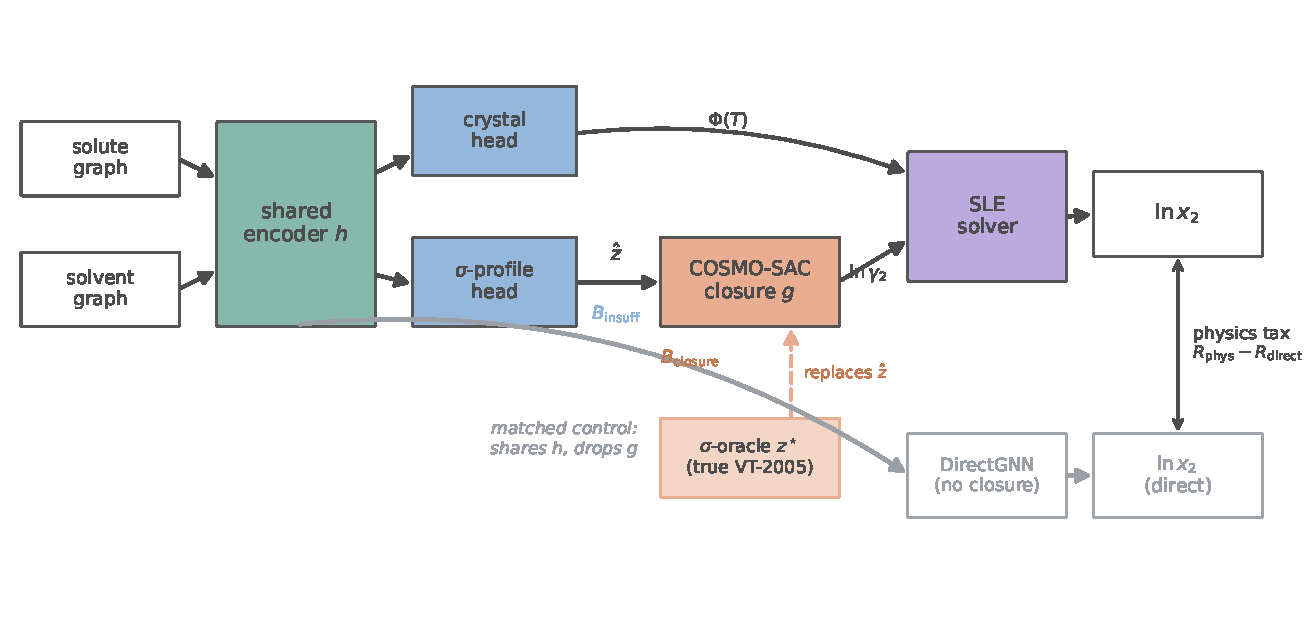
\includegraphics[width=0.82\linewidth]{figs/fig_architecture.pdf}
\caption{The model and the oracle substitution. Solute and solvent graphs pass
through a shared encoder to a crystal head (the ideal term $\Phi(T)$) and a
$\sigma$-profile head; the predicted profile $\hat z$ feeds the fixed COSMO-SAC closure
$g$, which returns $\ln\gamma_2$, and an SLE solver combines the two into $\lnx$. Input
insufficiency $\Binsuf$ enters at the intermediate $\hat z$ and closure misspecification
$\Bclos$ at $g$. The $\sigma$-oracle replaces $\hat z$ with the reference VT-2005 profile
$\zstar$ (salmon). DirectGNN (grey) is the capacity- and budget-matched control---it shares the
encoder but drops the closure; its optimisation settings were tuned separately (\S\ref{sec:framework}).}
\label{fig:arch}
\end{figure*}

\paragraph{Encoder backbones.} The shared encoder has three interchangeable backbones: the
headline message-passing network (MPNN); a hybrid local-message/global-attention graph transformer
(GPS \cite{rampasek2022}); and a physics-channelled variant, Thermodynamically-Informed Message
Passing (TIMP), which splits messages into dispersive, polar, and hydrogen-bonding channels
supervised toward the Hansen parameters to prevent channel collapse. TIMP does not outperform the plain
MPNN across our runs, consistent with the encoder being transfer-limited rather than
expressivity-limited (linear probe train $R^2\approx0.76$, test $R^2\approx0.45$).
\paragraph{Optimisation, and the two arms' settings.} The physics arm uses Adam (weight decay
$5\times10^{-4}$, gradient clipping at $2.0$, batch $64$)
under the three-phase curriculum of \S\ref{sec:methods}: $30$ epochs of auxiliary pretraining (P1),
$70$ of full SLE training (P2), and $10$ of low-rate stabilisation (P3), at learning rates
$2.6\times10^{-4}$, $8.5\times10^{-5}$, and $8.5\times10^{-6}$ respectively. The DirectGNN control
was tuned separately and its settings differ: dropout $0.174$ against $0.012$, P2 learning rate
$8.6\times10^{-4}$ against $8.5\times10^{-5}$, weight decay $4.2\times10^{-5}$ against
$5\times10^{-4}$, gradient clipping $2.54$ against $2.0$, over $110$ P2 epochs equal to the physics
arm's total budget at the same width ($64$) and depth ($3$). Width, depth, batch size and epoch
budget are therefore matched and the optimisation is not, so $\Delta_\infty$ and every per-arm
$\Delta\mathrm{MAE}$ in this paper is a difference between two separately tuned pipelines and is not
attributable to the thermodynamic bottleneck alone (\S\ref{sec:framework}). A
hyperparameter-matched control was not run.
\paragraph{Loss.} The objective is a weighted sum. Of its $32$ registered terms, $17$ carry weight
$0$ by default and never enter training---disabled experimental scaffolding (TIMP channel supervision;
van't~Hoff / temperature terms, $\times7$; Hansen-contrastive terms, $\times5$; descriptor/group priors;
an auxiliary direct-solubility term), released with the code for completeness. The $15$ \emph{active}
terms are below; only the top two groups are load-bearing for the claims, and a loss-simplification
ablation (\S\ref{sec:si-lossablation}) tests which.

\begin{table}[h]
\centering\small
\resizebox{\columnwidth}{!}{%
\begin{tabular}{@{}llr@{}}
\toprule
role & term & default wt. \\
\midrule
task                 & solubility (bin-weighted Huber on $\lnx$)        & $1.0$ \\
crystal grounding    & melting point $\Tm$                              & $0.3$ \\
                     & fusion enthalpy $\dHfus$                         & $0.3$ \\
$\sigma$/act.\ ground.& infinite-dilution $\lngi$                       & $0.5$ \\
                     & finite-composition $\lng$                        & $0.5$ \\
                     & Hansen parameters                                & $0.2$ \\
                     & $\sigma$-profile EMD (grounding stream on)        & $^\dagger$ \\
regulariser          & solubility monotonicity in $T$                   & $0.1$ \\
                     & physics preference                               & $0.1$ \\
                     & adaptive-correction residual                     & $0.01$ \\
                     & NRTL $\tau$                                       & $0.01$ \\
                     & solubility variance                              & cfg \\
control coupling     & DirectGNN NLL                                    & $0.2$ \\
                     & DirectGNN regulariser                            & $0.05$ \\
architecture         & mixture-of-experts balance                       & $0.02$ \\
\bottomrule
\end{tabular}}
\caption{The $15$ active loss terms (non-zero default weight). $^\dagger$The $\sigma$-profile
earth-mover term is active only when the grounding stream is on.
A further $17$ registered terms are disabled (weight $0$). Per-phase weight overrides are pinned in each
run's resolved configuration.}
\label{tab:loss}
\end{table}

\paragraph{Loss-simplification ablation.}\label{sec:si-lossablation}
For a diagnostic result the elaborate objective is a potential confound: the paradox
could be an artifact of loss tuning. We test the opposite---that the paradox and the compensating-surrogate
drift survive a \emph{minimal} objective. Pre-registered before the run: train the end-to-end grounded
arm with only the task ($\lnx$ Huber), the crystal grounding ($\Tm,\dHfus$), and the $\sigma$-profile
warmup, \emph{dropping} the activity-grounding auxiliaries ($\lngi$, $\lng$, Hansen) and every
regulariser, then read the sign of the paradox (oracle vs.\ learned) and the surrogate drift.
Prediction: both persist, because the mechanism is end-to-end training through a misspecified closure,
not the auxiliary terms. Confirmed at the level the ablation measures. The ablation re-measures the
solubility \emph{paradox} (reference minus learned $\lnx$ MAE), the observable effect, not the profile drift
directly: on the full test set it is $+1.13$ (95\% CI $[0.88,1.38]$) under the minimal objective,
\emph{larger} than the $+0.30$ ($[0.20,0.39]$) under the full one. This is the \emph{overall},
solvent-dominated paradox, and it strengthens once the activity-grounding auxiliaries---the only pressure
toward physics---are removed; on the both-reference subset ($n{=}297$ rows over the ${\approx}7$ VT-covered
solutes) the sign in fact reverses ($-0.23$ minimal vs $+0.22$ full), so the ablation is evidence
that the overall observable effect is loss-robust, not subset-level confirmation of the mechanism. It is
\emph{consistent with} the compensating surrogate being intrinsic to end-to-end training through a
misspecified closure rather than a regularisation artifact; it is an implication of the amplified paradox,
not a direct re-measurement of $\lVert\hat\sigma-\sigma\rVert$ under the minimal run (the minimal-loss
checkpoint was not retained, and the larger reference-arm error is consistent with more profile drift but
does not isolate it from closure-path recalibration). The minimal model trains normally (validation
$\lnx$ MAE $1.87$, within $0.1$ of the full-loss base), ruling out a degenerate-training reading
(seed $42$; \texttt{scripts/\allowbreak analysis/\allowbreak run\_loss\_ablation\_analysis.py}).

\section{Proofs}
\label{sec:si-proofs}

\begin{proof}[Proof of Lemma~\ref{prop:ident} (non-identifiability)]
Write $u=1/T$ and $h=\dHfus/\Rgas$, $u_m=1/\Tm$. At infinite dilution and with
$\Delta C_p=0$ the observable is
\[
\begin{aligned}
  \mu(u)=-\Phicry(u)-\lngi(u)&=-h(u-u_m)-(c+d\,u)\\
  &=-(h+d)\,u+(h u_m-c),
\end{aligned}
\]
using $\lngi(u)=c+d\,u$ (affine in $u$ by hypothesis). Thus $\mu$ depends on the
parameters $\theta=(\dHfus,\Tm,c,d)$ only through the pair
$(S,K)=(-(h+d),\,h u_m-c)\in\mathbb R^2$. The activity block spans this plane,
$\partial(S,K)/\partial c=(0,-1)$ and $\partial(S,K)/\partial d=(-1,0)$; hence for
\emph{any} crystal value $(h,u_m)$ and any target $(S,K)$ there is an activity pair
$d=-S-h$, $c=h u_m-K$ reproducing it. The likelihood level set therefore contains the
full two-dimensional family $\{(h,u_m)\}$, so $(\dHfus,\Tm)$ are unidentified.
Equivalently, the crystal score $\partial(S,K)/\partial h=(-1,u_m)$ lies in the span
of the activity columns, so profiling out $(c,d)$ annihilates it and
$\mathcal I_{\mathrm{eff}}(\dHfus)=0$. At finite dilution
$\lng(u)=\lngi(u)\,(1-x_2)^2$ adds $\lngi(u)\,(2x_2-x_2^2)=O(x_2)$, which is not
affine in $u$ because $x_2=x_2(u)$; the crystal score then has a component outside the
activity span of order $x_2$, so $\mathcal I_{\mathrm{eff}}(\dHfus)=O(x_2^2)>0$.
\end{proof}

\begin{lemma}[Class-dependent efficient information]\label{prop:semiparam}
Let the activity nuisance lie in a class $\mathcal H$ with tangent projection
$\Pi_{\mathcal H}$, and let $v=\partial\mu/\partial\dHfus$ be the crystal score.
The efficient information for $\dHfus$ is
$\mathcal I_{\mathrm{eff}}(\dHfus)=\sigma^{-2}\,\lVert v-\Pi_{\mathcal H}v\rVert^2$.
If $\mathcal H$ contains the crystal score's span $\{1,1/T\}$ (a free intercept and slope) then
$\Pi_{\mathcal H}v=v$ and $\mathcal I_{\mathrm{eff}}=0$, recovering
Lemma~\ref{prop:ident}; if $\mathcal H$ is restricted (the slope is known or
constrained) then $\mathcal I_{\mathrm{eff}}>0$ and the Cram\'er--Rao lower bound (CRLB) on
$\dHfus$ is finite. (The melting point $\Tm$ is likewise an unknown crystal parameter, but is
profiled jointly: its score $\partial\mu/\partial\Tm$ lies in $\mathrm{span}\{1\}\subset
\mathrm{span}\{1,1/T\}$, already inside the nuisance tangent whenever the slope is free, so the
dichotomy is unaffected by treating $\Tm$ as free.)
\end{lemma}
\begin{proof}[Proof of Lemma~\ref{prop:semiparam} (class-dependent information)]
This is the semiparametric efficient-score construction \cite{vandervaart1998}
(here finite-dimensional and Gaussian, so equivalently the partitioned-information /
Frisch--Waugh--Lovell identity). With
Gaussian noise of variance $\sigma^2$, parameter-of-interest score
$v=\partial\mu/\partial\dHfus$, and nuisance tangent space $\mathcal T_{\mathcal H}$
(the $L^2$-closure of the span of nuisance scores), the efficient score is the
residual $\tilde v=v-\Pi_{\mathcal H}v$ and the efficient information is
$\mathcal I_{\mathrm{eff}}=\sigma^{-2}\lVert v-\Pi_{\mathcal H}v\rVert^2$. Here
$v=\partial\mu/\partial\dHfus=-(u-u_m)/\Rgas\in\operatorname{span}\{1,u\}$. If
$\mathcal T_{\mathcal H}\supseteq\operatorname{span}\{1,u\}$ then $\Pi_{\mathcal H}v=v$
and $\mathcal I_{\mathrm{eff}}=0$, recovering Lemma~\ref{prop:ident}; if
$\mathcal T_{\mathcal H}$ is a proper subspace not containing $v$ (e.g.\ a fixed
slope, $\mathcal T_{\mathcal H}=\operatorname{span}\{1\}$) then
$\Pi_{\mathcal H}v\neq v$ and $\mathcal I_{\mathrm{eff}}>0$, with a finite
Cram\'er--Rao bound.
\end{proof}

\begin{proof}[Proof of Lemma~\ref{prop:decomp} (decomposition and bounds)]
\emph{(a) Identity.} Split the residual as
$m-g(\zstar)=[m-\Ex(m\mid\zstar)]+[\Ex(m\mid\zstar)-g(\zstar)]$, square, and take
expectations. The squared terms give $\Ex[\Var(m\mid\zstar)]=\Binsuf$ and
$\Ex[(\Ex(m\mid\zstar)-g(\zstar))^2]=\Bclos$. The cross term vanishes: since
$\Ex(m\mid\zstar)-g(\zstar)$ is $\sigma(\zstar)$-measurable, the tower rule gives
$\Ex\big[(m-\Ex(m\mid\zstar))(\Ex(m\mid\zstar)-g(\zstar))\big]
=\Ex\big[(\Ex(m\mid\zstar)-g(\zstar))\,\Ex(m-\Ex(m\mid\zstar)\mid\zstar)\big]=0$.
\emph{(b) Jensen lower bound.} With $\Delta(\zstar)=\Ex(m\mid\zstar)-g(\zstar)$,
$\Bclos=\Ex[\Delta^2]\ge(\Ex[\Delta])^2=(\Ex[m]-\Ex[g])^2$ by Jensen, using
$\Ex[\Ex(m\mid\zstar)]=\Ex[m]$; it requires only that $m$ and $g$ share a reference
state, so that $\Ex[m]-\Ex[g]$ is a genuine mean discrepancy.
\emph{(c) Law-of-total-variance upper bound.} For any binning
$B=\mathrm{bin}(g(\zstar))$, $\sigma(B)\subseteq\sigma(\zstar)$, so conditioning on the
coarser $\sigma$-algebra cannot reduce expected conditional variance:
$\Ex[\Var(m\mid B)]\ge\Ex[\Var(m\mid\zstar)]=\Binsuf$.
\emph{(d) Convention-independence.} $\Binsuf=\Ex[\Var(m\mid\zstar)]$ is a functional of
the law of $(m,\zstar)$ alone and does not involve $g$; hence it is identical across
closure conventions, and any $\mathrm{MSE}(g_1)-\mathrm{MSE}(g_2)$ is entirely
$\Bclos(g_1)-\Bclos(g_2)$.
\end{proof}

\begin{theorem}[Grounding-gap sandwich]\label{thm:gap}
Assume all risks are finite ($m,g(\zstar)\in L^2$; $g$ and each $h\in\mathcal E$
measurable), (A1) the true encoder is representable, $\phi^\star\in\mathcal E$ with
$\zstar=\phi^\star(x)$, and (A2) the intermediate is a lossless bottleneck,
$\Ex[m\mid x]=\Ex[m\mid\zstar]$. Then
\begin{equation}
0\;\le\;\Gamma\;\le\;\Bclos,\qquad
\Gamma=\Bclos-\big(R_{\mathrm{e2e}}-R_{\mathrm{free}}\big),
\label{eq:gap}
\end{equation}
with $\Gamma=\Bclos$ iff $R_{\mathrm{e2e}}=R_{\mathrm{free}}$ (the composed class realizes
the Bayes predictor by distorting the intermediate). In particular a well-specified closure
($\Bclos=0$) gives $\Gamma=0$; hence \emph{under A1--A2}, $\Gamma>0$ certifies $\Bclos>0$.
\end{theorem}
\begin{proof}[Proof of Theorem~\ref{thm:gap} (grounding-gap sandwich)]
Throughout assume $m,g(\zstar)\in L^2$ and $g$, every $h\in\mathcal E$ measurable.
\emph{(a) $\Gamma\ge0$.} By A1, $\phi^\star\in\mathcal E$ is a feasible encoder with
$g(\phi^\star(x))=g(\zstar)$, so $R_{\mathrm{e2e}}=\inf_{h}\Ex[(m-g(h(x)))^2]\le
\Ex[(m-g(\zstar))^2]=R_{\mathrm{orc}}$; the infimum need not be attained. Hence
$\Gamma=R_{\mathrm{orc}}-R_{\mathrm{e2e}}\ge0$.
\emph{(b) $R_{\mathrm{e2e}}\ge R_{\mathrm{free}}$.} Every $g(h(x))$ is
$\sigma(x)$-measurable, and $R_{\mathrm{free}}=\Ex[(m-\Ex(m\mid x))^2]$ is the infimum of
$\Ex[(m-p)^2]$ over \emph{all} $\sigma(x)$-measurable $p$; an infimum over the subclass
$\{g(h(\cdot)):h\in\mathcal E\}$ is no smaller.
\emph{(c) $R_{\mathrm{free}}=\Binsuf$ under A2.} From
$\Var(m)=\Ex[\Var(m\mid x)]+\Var(\Ex(m\mid x))=\Ex[\Var(m\mid\zstar)]+\Var(\Ex(m\mid\zstar))$
and A2 ($\Ex(m\mid x)=\Ex(m\mid\zstar)$, so the two $\Var(\Ex(\cdot))$ terms agree), the two
expected conditional variances agree: $R_{\mathrm{free}}=\Ex[\Var(m\mid x)]=\Binsuf$.
\emph{(d) Sandwich and identity.} By Lemma~\ref{prop:decomp},
$R_{\mathrm{orc}}=\Binsuf+\Bclos$. With (c),
$\Gamma=R_{\mathrm{orc}}-R_{\mathrm{e2e}}=\Bclos-(R_{\mathrm{e2e}}-R_{\mathrm{free}})$, and (b)
gives $R_{\mathrm{e2e}}-R_{\mathrm{free}}\ge0$, so $0\le\Gamma\le\Bclos$; equality
$\Gamma=\Bclos$ holds iff $R_{\mathrm{e2e}}=R_{\mathrm{free}}$. Finally $\Bclos=0$ forces
$0\le\Gamma\le0$, i.e.\ $\Gamma=0$; contrapositively, under A1--A2, $\Gamma>0\Rightarrow\Bclos>0$.
\emph{(e) A2 is necessary for the certificate.} If A2 fails, take $x\in\{a,b\}$ equiprobable,
$\zstar\equiv0$ (so A1 holds), $m(a)=+1,m(b)=-1$, and $g$ with $g(0)=0=\Ex(m\mid\zstar)$ so
$\Bclos=0$; an encoder $h^\dagger(a)=1,h^\dagger(b)=-1$ with $g(\pm1)=\pm1$ gives
$R_{\mathrm{e2e}}=0$ while $R_{\mathrm{orc}}=1$, hence $\Gamma=1>0=\Bclos$. So $\Gamma>0$ alone
does not certify $\Bclos>0$; the decomposition (Lemma~\ref{prop:decomp}) does.
\end{proof}

\noindent The penalty-sign result (Proposition~\ref{prop:tax}, stated in the main text at
\S\ref{sec:tax}) is proved here.
\begin{proof}[Proof of Proposition~\ref{prop:tax} (sign of the physics penalty)]
\sloppy\relpenalty=0 \binoppenalty=0
Write $D(n):=V_{\mathrm{direct}}(n)-V_{\mathrm{phys}}(n)$ and
$\Delta_\infty:=R_{\mathrm{e2e}}-R_{\mathrm{direct},\infty}$, so that
$\mathcal{T}(n)=\Delta_\infty-D(n)$.
\emph{(i)} $\mathcal{T}(n)<0$ exactly when $D(n)>\Delta_\infty$, immediately.
\emph{(ii)} If $\Delta_\infty>0$ and $D(n)\to0$, choose $n^\star$ with $|D(n)|<\Delta_\infty$
for all $n>n^\star$ (possible since $D(n)\to0$); then $\mathcal{T}(n)=\Delta_\infty-D(n)>0$. Monotonicity
of $D$ is \emph{not} required for existence of $n^\star$; it is needed only for the stronger
claim ``$\mathcal{T}(n)>0$ at every $n$,'' which we treat as an empirical observation.
\emph{(iii)} Since $V_{\mathrm{phys}}(n)\ge0$, $D(n)\le V_{\mathrm{direct}}(n)$: the variance a
prior can save is bounded by the control's own estimation variance. As the black box approaches
the aleatoric floor $V_{\mathrm{direct}}(n)\to0$, so $\limsup_n D(n)\le0$; with both estimators
consistent, so $V_{\mathrm{phys}},V_{\mathrm{direct}}\to0$, one has $D(n)\to0$ and
$\mathcal{T}(n)\to\Delta_\infty\ge0$. When the control is asymptotically Bayes, so
$R_{\mathrm{direct},\infty}=R_{\mathrm{free}}$, and A2 holds, then
$\Delta_\infty=R_{\mathrm{e2e}}-R_{\mathrm{free}}=\Bclos-\Gamma$ by \eqref{eq:gap}.
\end{proof}


\section{Per-arm tables and decomposition robustness}
\label{sec:si-tables}
Table~\ref{tab:si-arms} gives the exact per-arm metrics behind
Fig.~\ref{fig:paradox}: three seeds (mean$\pm$sd) on the cross-arm intersection lock
($n{=}5608$, rows supervised and finite in every arm). Both closure families---NRTL and
COSMO-SAC over a learned $\sigma$-profile---trail the DirectGNN control (the physics
penalty); the $\sigma$-oracle (reference VT-2005 profile) is the worst arm, and restoring the
Staverman--Guggenheim combinatorial term makes it slightly worse still---the signature
of a misspecified map (\S\ref{sec:measure}).

\begin{table*}[h]
\centering
\caption{Per-arm scaffold-split metrics (3 seeds, $n{=}5608$ cross-arm lock).
Ordered by MAE.}
\label{tab:si-arms}
\begin{tabular}{lrr}
\toprule
Arm & MAE & $R^2$ \\
\midrule
DirectGNN (no closure)                         & $1.70\pm0.03$ & $+0.42\pm0.03$ \\
NRTL closure                                   & $1.80\pm0.07$ & $+0.34\pm0.03$ \\
COSMO-SAC, learned $\sigma$ (grounded)         & $1.85\pm0.05$ & $+0.33\pm0.05$ \\
\quad $+$ Staverman--Guggenheim combinatorial  & $1.88\pm0.09$ & $+0.32\pm0.05$ \\
COSMO-SAC, ungrounded $\sigma$                 & $2.04\pm0.04$ & $+0.19\pm0.01$ \\
COSMO-SAC, reference $\sigma$ ($\sigma$-oracle)     & $2.25\pm0.02$ & $-0.03\pm0.04$ \\
\bottomrule
\end{tabular}
\end{table*}

% Schedule: configs/cosmo_sac.yaml (freeze_sigma_head_during_sle, warmup 40, 30/70/10 epochs)
% + scripts/experiments/run_e5_sigma_grounding.sh (per-arm invocations).
\paragraph{$\sigma$-head schedule of these arms.} The four COSMO-SAC rows come from three
training runs under one pinned configuration --- $30$ P1, $70$ P2 and $10$ P3 epochs with
\texttt{freeze\_sigma\_head\_during\_sle} on, so the $\sigma$ head's weights are held from P2
onward. The two grounded rows precede that with a $\sigma$ warm-up on the grounding pool (up to $40$
epochs, early-stopped on a held-out tenth of the pool) and interleave the pool through P1; under the
freeze the stream is inactive in P2/P3. The ungrounded row sets warm-up and stream budget to zero,
so its $\sigma$ head is shaped in P1 by the corpus-internal \lngi\ auxiliary loss alone, never by an
external $\sigma$ label, and is frozen from P2 in the same way. The $\sigma$-oracle row is the grounded
checkpoint re-evaluated with $\zstar$ injected, so it shares the grounded schedule exactly. Because
the freeze holds the head and not the encoder that feeds it, the predicted profile is not pinned at
its warm-up value in these arms; we have not run the surrogate isolation (\S\ref{sec:surrogate}) on
these checkpoints, so how far their latent drifted is not measured, and the supervision contrast
quoted there ($+0.40\to+0.14$) is a separate matched pair of runs --- one warm-up-plus-short-P1 base
resumed twice for SLE, with the freeze off and on, on $n{=}5571$ matched rows --- and not these arms.

% Artifacts: results/e5_sigma_grounding/seed_42/{grounded_a_truetrain,channel_swap}_predictions.csv
% (seed 42 only; no seed_43/seed_44 counterpart), scored on the same n=5608 cross-arm lock.
\paragraph{Oracle-application controls: two of the three are single-seed.} Of the three oracle
applications (\S\ref{sec:methods}), only the evaluation-only substitution is a three-seed result.
Training-time injection (MAE $1.98$) and the channel swap (MAE $2.08$) were run at seed $42$ alone,
so their matched comparator is the seed-$42$ learned-$\sigma$ value $1.80$ on the same $n{=}5608$
lock, not the three-seed mean $1.85$ of Table~\ref{tab:si-arms}. Both exceed the worst of the three
learned-$\sigma$ seeds ($1.80/1.92/1.81$), so the direction of both survives a worst-case seed
comparison. The channel-swap margin ($+0.28$) is $2.3$ times the learned arm's full between-seed
range; the training-time margin ($+0.18$) is one and a half times it, so that control fixes a sign
rather than an effect size.

\paragraph{Robustness of the closure/insufficiency separation.} We stress-test the deployed-convention verdict
$\Bclos>\Binsuf$ (\S\ref{sec:measure})---equivalently $\Binsuf<\mathrm{MSE}/2=0.74$ at
$\mathrm{MSE}_{\mathrm{res}}=1.47$---four ways on the $n{=}60$ set.

\emph{(i)~Estimator sensitivity.} The four $\Binsuf$ upper bounds of Table~\ref{tab:decomp}---$0.40$
($k$-NN), $0.62$ (binning/LOTV), $0.56$ (random forest), $0.62$ (ridge out-of-fold)---all fall below the
$0.74$ threshold. The $k$-NN value is the smallest and least conservative input to $\Bclos\ge\mathrm{MSE}-\Binsuf^{\mathrm{up}}$,
so we take the leakage-immune LOTV bound as the headline instead. The LOTV bound bins $g(\zstar)$ and is therefore
finite-sample downward-biased when points per bin are few, which would \emph{inflate} $\Bclos$ favourably;
The two non-binning bounds (RF $0.56$, ridge $0.62$) are immune to that particular per-bin sparsity,
but they do not provide independent corroboration: under random folds every held-out row shares its
solvent or its solute with a training row, so both can borrow strength from a near-twin,
anti-conservatively and in the same direction as the binning (\S\ref{sec:measure}). Blocking folds on
both molecules leaves no informative estimator on this set. The headline should therefore be read as
resting on the leakage-immune LOTV bound alone, not on agreement between three estimators.
The sole non-certifying configuration is a
deliberately aggressive ridge, which lifts $\Binsuf$ to $0.88$ (then $\Bclos\ge0.59<0.88$): a sensitivity
edge, not a refutation.

\emph{(ii)~Leave-one-solvent-out.} Dropping each of the $17$ solvents in turn, the verdict holds in all
$17$ folds under the LOTV bound. Under the random-forest estimator it holds in only $2/17$, because an RF
over-fits conditional variance in $102$ dimensions at $n{=}60$ (its out-of-fold MSE approaches $\Var(m)$),
so its leave-one-out estimate is unstable---an estimator artifact, not a sign flip.

\emph{(iii)~Label noise.} Injecting zero-mean Gaussian noise $\sigma_\eta\in\{0.2,\dots,0.8\}$ into $m$
leaves the $\Bclos$ lower bound stable ($0.84\to0.70$), as expected since
$\Bclos=\mathrm{MSE}-\Ex[\Var(m\mid\zstar)]$ is invariant to zero-mean noise.

\emph{(iv)~Clustered-bootstrap interval.} A solvent-clustered bootstrap ($3000$ resamples of the $17$
solvents, LOTV bound) makes the confidence explicit: the $\Bclos$ lower bound has median $0.93$
(CI$_{90}$ $[0.40,\,1.62]$), and the margin $\Bclos-\Binsuf$ has median $0.36$ (CI$_{90}$ $[-0.22,\,+0.97]$)
with $P(\Bclos>\Binsuf)\approx0.89$ (single-axis; the conservative two-way solute$\times$solvent bootstrap,
which also charges for repeated solutes, gives $\approx0.78$, the value reported in the main text). With
$G=17$ solvent and $41$ solute clusters this small-$G$ regime has optimistic interval coverage, and the
finite-cluster correction acts in the direction of less confidence and non-certification. We
therefore treat the $P$ values as a coarse band, not two-decimal quantities. The separation is
\emph{likely} but not certified at the $90\%$ level under either clustering, which is
why the main text treats it as supporting rather than decisive.

\paragraph{In-regime ($\gamma$-stratified) separation.} The $n{=}60$ measurement is matched at low $\gamma$,
while the paradox spans all $\gamma$. Stratifying the $n{=}60$ set by $\lngi$
tests whether closure-dominance is a regime artifact. It is
not: the verdict $\Bclos>\Binsuf$ (leakage-immune LOTV binning bound) holds in every
stratum and \emph{strengthens} toward higher $\gamma$ (Table~\ref{tab:regime})---in the highest
stratum ($\overline{\lngi}=2.94$, approaching the non-ideal regime) $\Bclos\ge2.69$ exceeds
$\Binsuf\le0.67$ several-fold. The high-$\gamma$ strata are small
($n=17$--$30$ in $102$ dimensions): the law-of-total-variance bound can be pushed toward zero by
too-few-points-per-bin, which mechanically widens the margin exactly where data is thinnest, so
it is the several-fold separations rather than the precise values that carry the
qualitative reading. The bound here bins each stratum into three equal-count bins (against eight in
the main text) and uses the maximum-likelihood within-bin variance, as in the
headline row of Table~\ref{tab:decomp}; recomputed with the unbiased (Bessel) one it rises to
$0.08/0.95/0.81$ across the three strata, so each still separates, but the middle stratum only
marginally ($0.95$ against its own $\mathrm{MSE}/2=0.96$). The $m>\overline{m}$ stratum separates
through its upper (high-$\gamma$) half, and the \emph{isolated} moderate band
($\overline{m}<m\le1.5$) does \emph{not} separate. This is not a counter-example. The total error there
is only ${\approx}0.06$, so $\Bclos\le\mathrm{MSE}\approx0.06$ assumption-free (since $\Binsuf\ge0$),
and there is simply nothing to attribute---near ideality the target is small and the split is
uninformative. We read no closure-quality claim from it in either direction. This supports---but does
not prove---the conjecture that the same closure misspecification drives the all-$\gamma$ paradox.

\begin{table}[h]
\centering
\caption{Closure/insufficiency verdict across $\lngi$ strata of the matched set (deployed
residual-only convention; $\Binsuf^{\mathrm{up}}$ is the leakage-immune LOTV binning bound throughout,
at the maximum-likelihood within-bin variance).}
\label{tab:regime}
\resizebox{\columnwidth}{!}{%
\begin{tabular}{lrrrr}
\toprule
Stratum & $n$ & $\overline{\lngi}$ & $\Binsuf\le$ & $\Bclos\ge$ \\
\midrule
lower $\gamma$ ($m\le$ med.) & $30$ & $-0.40$ & $0.08$ & $0.95$ \\
higher $\gamma$ ($m>$ med.)  & $30$ & $+1.90$ & $0.86$ & $1.07$ \\
high $\gamma$ ($m>1.5$)      & $17$ & $+2.94$ & $0.67$ & $2.69$ \\
\bottomrule
\end{tabular}}
\end{table}

The closure/insufficiency decomposition (full/res conventions; law-of-total-variance (LOTV), random-forest (RF), ridge, and
k\textsc{nn} estimators; solvent-clustered bootstrap; the pyridine stratum) is
tabulated in \S\ref{sec:measure}.

\begin{figure}[t]
\centering
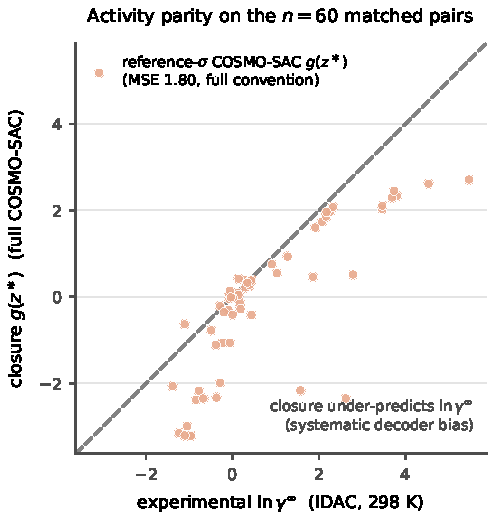
\includegraphics[width=0.72\linewidth]{figs/fig_parity.pdf}
\caption{Activity-coefficient parity on the $n{=}60$ matched pairs. The reference-$\sigma$
COSMO-SAC closure $g(\zstar)$ (salmon) falls below the diagonal at
larger $\lngi$, under-predicting the activity coefficient (MSE $1.80$, full
convention).}
\label{fig:parity}
\end{figure}

\paragraph{The four hedges (full).} The adversarial audit does not invert the verdict
but sharpens its scope:
\begin{enumerate}
  \item \emph{Convention.} The deployed default is residual-only. Under it the
  \emph{constant-offset} (Jensen) lower bound inverts
  ($\Bclos\ge0.43<\Binsuf\le0.62$; it separates only under the full convention,
  $\Bclos\ge0.72$), so that assumption-free bound does not separate under deployment
  (this is the convention-specific row deferred here from Table~\ref{tab:decomp} /
  Fig.~\ref{fig:decomp}), and
  the full-convention margin (the sharpened $\mathrm{MSE}-\Binsuf$ bound,
  $1.27$ vs $0.53$) is a full-COSMO-SAC-only result. What separates under the deployed
  convention is the leakage-immune bound
  $\Bclos\ge\mathrm{MSE}_{\mathrm{res}}-\Binsuf^{\mathrm{LOTV}}\approx0.85>0.62$, which carries
  the headline claim, together with the combinatorial argument above.
  \item \emph{Confound.} The closure error is predominantly a \emph{between-solvent}
  systematic bias ($\sim$64\% of total error); within the largest single-solvent stratum
  (pyridine, $n{=}20$) the closure is nearly correct (stratum MSE $0.07$). Because
  solvent $\sigma$ is part of $\zstar$, these offsets are still decoder error and give an
  independent solvent-conditional lower bound $\Bclos\ge0.89$ (full)/$0.56$ (res).
  \item \emph{Confidence.} Confidence on the full-convention constant-offset
  separation is the solvent-clustered bootstrap $P(\Bclos{>}\Binsuf)\approx0.85$ ($0.83$
  vs the random-forest upper bound, $0.89$ vs the law-of-total-variance bound); we report
  the solvent-clustered scheme rather than the less conservative i.i.d.-pair one because
  solvent dependence dominates. The leakage-immune margin ($0.85$ vs $0.62$) is a
  point estimate. The decomposition is checkpoint/seed-independent (the closure has zero
  learnable parameters).
  \item \emph{Selection/scope.} The 60 matchable pairs are the low-to-moderate $\gamma$
  regime (matched mean $\lngi=0.75$ vs $3.56$ for VT-2005-unmatchable pairs, $t=-7.44$;
  the strongly non-ideal amide-solvent regime is untested because VT-2005 lacks those
  profiles). This narrows scope but is \emph{conservative}, since the untested regime is
  a harder closure test. The target is $\lngi$ at 298\,K, so the numeric ceiling does not
  necessarily transfer unchanged to the finite-composition solubility regime.
\end{enumerate}

\section{External baselines and ablations}
\label{sec:si-baselines}
% Artifacts: results/external_baselines/solute/{fastsolv,solprop_calibrated,solprop_native}_contract_v2/metrics.json.
We evaluated the direct state-of-the-art model (FastSolv \cite{osanloo2024}) and the
physics-informed state-of-the-art model (SolProp \cite{vermeire2022solprop}) on a
by-solute test split (\texttt{test\_solute.csv}, $n\approx10$--$12$k). The two arms are not obtained
the same way, and the difference matters below: FastSolv is retrained on our corpus, whereas SolProp
is the released pretrained thermodynamic cycle---the arm that instantiates the physics---mapped onto
our target by a three-parameter linear recalibration fitted on the training rows, not by retraining.
That cycle is run at $298$\,K on every row, so the temperature of a measurement reaches the SolProp
arm only through the calibrator's temperature term. In $\lnx$ they
reach MAE $1.94$ (FastSolv, $R^2\,0.23$) and $2.34$ (SolProp, calibrated,
$R^2\,{-}0.18$); in $\log_{10}S$, $0.87$ and $1.04$. These are on a \emph{by-solute} split that is
\emph{not comparable} to our scaffold numbers (Table~\ref{tab:si-arms}): they bound the task's
difficulty, not a ranking of the models against one another, so this does \emph{not} establish that our
scaffold-split DirectGNN ($1.70$) outperforms them; a like-for-like scaffold evaluation of the
external models was not run, the deposited external runs being by-solute and pair-random only.
The internal ordering---the physics-informed SolProp trailing the direct FastSolv, the same
ordering we find between our physics closures and DirectGNN---is therefore a
comparison of the \emph{cycle} against a direct model, and it reverses when SolProp's encoder is
instead retrained directly on $\lnx$ with the cycle discarded: that arm reaches MAE $1.63$
($R^2\,0.39$) in $\lnx$ and $0.76$ in $\log_{10}S$ on the $n{=}10{,}287$ rows FastSolv is scored on,
against FastSolv's $1.94$ and $0.87$. We quote the cycle as the physics-informed arm because only it
assembles the separately learned components; the retrained arm measures what discarding the closure
buys on this corpus, not a better physics-informed model. The regime-level reading is that on this corpus no
black box, ours or external, escapes the accuracy ceiling---consistent with the
structural account of \S\ref{sec:discussion}. Per-arm ablations (NRTL vs COSMO-SAC,
combinatorial on/off) are in Table~\ref{tab:si-arms}.

\section{Supplementary mechanism results}
\label{sec:si-mech}
\paragraph{Non-identifiability, empirically (the corrupted twin).} Training a twin model
on data whose crystal labels are corrupted (every $\Tm$ shifted by $+273$\,K) leaves the
\emph{solubility} fit essentially unchanged---$\lnx$ MAE $1.835$ versus $1.812$ on the
corrected data---while the recovered crystal grounding differs by hundreds of kelvin
($\Tm$ MAE $258$\,K versus $45$\,K). Two very different crystal/activity splits produce
the same solubility, which is Lemma~\ref{prop:ident} made concrete.
\paragraph{Crystal grounding on physical labels.} When the crystal head is supervised
on measured melting points it predicts $\Tm$ to $45$\,K MAE, about $4\times$ better than
a Joback group-contribution reference---so the flat downstream result of
\S\ref{sec:e2} is a dose/identifiability effect, not an inability to learn crystal
properties.
\paragraph{The $\Delta C_p=0$ approximation.} The ideal term omits the constant-heat-
capacity correction; a group-contribution audit finds a nonzero $\Delta C_p$ for
$1441$ of $1525$ solutes ($108{,}287$ rows), so this is a bounded model-form
approximation. It cannot produce either headline result. The closure/insufficiency
decomposition is measured on the activity target ($\lngi$ at $298$\,K), where $\Delta C_p$
does not enter at all; and the grounding paradox is an arm-to-arm difference (learned-$\sigma$
vs.\ oracle-$\sigma$) whose two arms share the \emph{identical} crystal term, so any $\Delta C_p$
error cancels exactly in the comparison. It is thus orthogonal to the activity closure, not a
source of the paradox.
\paragraph{Fusion-supervision scarcity.} Direct $\dHfus$ labels are extremely sparse:
$1279$ training rows across $31$ solutes, and essentially none in validation or test.
This is the quantitative basis of the identifiability argument---there is almost no
signal with which to pin the crystal term from data.
\paragraph{The NRTL branch trains (a trainability check).} The asymptotic physics penalty is not an
under-training artifact of the activity branch. In the headline NRTL arm the head produces
solvent-varying interaction parameters---$\tau_{12}$ over the $n{=}8103$ test pairs has mean
$0.97$ and std $2.5$ (range $[-2.6,22]$), far from collapsed---yet the arm still trails the
closure-free DirectGNN ($1.80$ vs $1.70$; Table~\ref{tab:si-arms}). A trained, non-degenerate
activity branch that the control still outperforms is evidence that the penalty is structural, not a
failure to train the branch.
(The core closure-misspecification result---the $\sigma$-oracle and the decomposition---is in
any case training-\emph{independent}: it feeds the reference VT-2005 profiles through the fixed
closure with no encoder optimization, so it cannot be a training pathology.)

\paragraph{Structured temperature extrapolation.} Withholding \emph{temperature} rather
than structure (train at $T\le309.75$\,K, test at higher $T$; $n=3343$), the
affine-in-$1/T$ hypothesis classes extrapolate far better than an unstructured
descriptor regressor (Table~\ref{tab:si-temp}); the van't~Hoff class also predicts the
\emph{direction} of the high-$T$ shift correctly $99\%$ of the time versus $40\%$ for
the random forest. This is a property of the structured hypothesis class---the trained
neural models are weaker than the van't~Hoff baseline---not an accuracy claim for our
model.

\begin{table}[h]
\centering
\caption{Same-pair high-temperature extrapolation ($n=3343$, train $T\le309.75$\,K).
``dir.'' is the fraction of pairs whose high-$T$ shift direction is predicted
correctly.}
\label{tab:si-temp}
\begin{tabular}{lrrr}
\toprule
Model & MAE & $R^2$ & dir. \\
\midrule
per-pair van't~Hoff ($1/T$)     & $0.37$ & $0.89$ & $0.99$ \\
per-pair linear in $T$          & $0.41$ & $0.85$ & $0.99$ \\
per-pair last-low-$T$ hold      & $1.20$ & $0.69$ & $0.01$ \\
RF (Morgan $+\,T$)              & $1.29$ & $0.66$ & $0.40$ \\
per-pair mean                   & $1.46$ & $0.56$ & $0.01$ \\
\bottomrule
\end{tabular}
\end{table}

\section{Supplementary diagnostics and broad negatives}
\label{sec:si-diagnostics}
\subsection{Supporting diagnostics} \label{sec:supporting}

The interpretive claims of the preceding sections are based on a set of controlled diagnostics, each run under a named protocol. We report them here with their exact numbers, including the results that are unfavourable to the physics-informed hypothesis.

% NOISE FLOOR: the derivation, both functionals and every value moved into the article at
% \S\ref{sec:data} on 2026-08-02 (editorial item A3) -- the referees asked for it there and it is
% one of the four things they could not verify without this document. What is left here is the
% part the article does not carry: the upper tail of the per-group distribution, which is what
% says the floor's mean is set by a minority of badly disagreeing systems.
\paragraph{Aleatoric noise floor.} The derivation, the two aggregating functionals and their values
are in the article at \S\ref{sec:data}. One property of the per-group distribution is not: it is
strongly right-skewed, which is why the mean and the median differ by a factor of five. On the
groups backed by two sources the $90$th percentile of the per-group disagreement is $0.42$ \lnx{}
units and the $99$th is $1.41$; on those backed by three, $0.83$ and $3.55$. The floor's
mean is therefore set by a minority of badly disagreeing systems rather than by a broad band, and on
either reading it lies far below the scaffold-split error.

\paragraph{The encoder is transfer-limited, not expressivity-limited.} To separate what the frozen graph embedding can represent from what it transfers out of distribution, we fit a linear probe from the encoder representation onto RDKit descriptors and compare in-distribution and held-out fit. The median train $R^2$ is $0.758$ against a test $R^2$ of $0.448$ ($n=700$ solutes in each partition), a gap of $0.31$. Individual descriptors split sharply: FractionCSP3 transfers well (test $R^2 = 0.96$) while HeavyAtomCount does not ($0.23$). The embedding is expressive enough in sample; what degrades out of distribution is the generalisation of that expressivity across scaffolds. This evidence is suggestive rather than decisive: the sharp per-descriptor spread (FractionCSP3 $0.96$ vs HeavyAtomCount $0.23$) means the train--test gap partly reflects covariate shift in the descriptor \emph{targets} across scaffolds rather than an encoder property alone, and the probe measures descriptor-representability, not task-relevant expressivity directly. It therefore \emph{suggests}---rather than establishes---that a new graph encoder is unlikely to be the main lever for out-of-distribution accuracy, with pretraining and coverage the more likely ones.

\paragraph{Temperature extrapolation.} A structured van't Hoff activity class (log-solubility affine in $1/T$) encodes the correct temperature dependence of \lng{} by construction, and this is apparent when the split withholds temperature rather than structure. Training on measurements at $T \le 309.75$~K and testing at $T \ge 330$~K ($n_{\text{test}} = 3343$), the structured class attains a high-temperature MAE of $0.37$ against $1.29$ for a random forest over Morgan fingerprints plus temperature (in \lnx{} units), consistent with the temperature-aware \lngi{} modelling of \cite{sanchezmedina2023}. This is a property of the structured hypothesis class, not a performance claim for the trained model: the functional form carries temperature extrapolation that a descriptor-plus-temperature regressor does not. Neither is it a claim that our trained arms fail to carry it. The one checkpoint scored on this split is a near-constant predictor whose activity branch never left initialisation, so it separates nothing (\S\ref{sec:si-mech}); what would separate it is a retraining of both arms on this split at the budget used elsewhere here.

% REPLACED 2026-08-06.  What stood here was a single-arm table -- rho 0.511 / top-1 0.477 /
% Kendall 0.436 / nDCG@3 0.732 at n=826 -- computed from
% results/e0_compensation/tgnn_mpnn_test_predictions.csv, an early proxy checkpoint on a
% SUPERSEDED split (826 groups, 5826 rows, against the current 823 and 5608).  It belonged to no
% arm of Fig. 2 and sat one paragraph from the arms a reader would take it for.  It is replaced,
% not annotated, by the paired within-checkpoint contrast of \S\ref{sec:paradox}, which measures
% the same thing on the arms this paper is about.  The retired values are recorded in
% paper/retired_numbers.txt.  The conformal sentence below comes from the same proxy checkpoint
% and now says so.
\paragraph{Ranking and calibration.} Absolute error and decision quality diverge, and within one
checkpoint the divergence has a direction. Table~\ref{tab:ranking} ranks the solvents of each
solute--temperature group of the labelled test rows under the two $\sigma$-profiles of
\S\ref{sec:paradox}: the same weights, the same rows, and only the profile fed to the closure
differing ($\max|\Delta\Phi|=4.2\times10^{-4}$ at the worst of the three seeds, against $4.4$ to
$5.9$ between separately trained arms). With its own learned profile the model orders solvents above
two solute-blind references; with the reference profile substituted it is not distinguishable from
either, on any of the four metrics, at any of the three seeds. Both arms remain far above the
within-group permutation floor, so the substitution does not reduce the ordering to chance---it
reduces it to one that a ranker never shown the solute could produce. Groups are formed on solute
and temperature rounded to $1$\,K, kept when they hold at least three distinct solvents, with
duplicate measurements averaged per solvent. The effective
sample is the $107$ solute clusters, not the $823$ groups, and every interval below is a $95\%$
bootstrap over those clusters.

\begin{table*}[t]
\centering
\caption{Solvent ranking under the two $\sigma$-profiles, on the labelled test rows grouped by
solute and temperature ($823$ groups, $107$ solute clusters, $\ge3$ solvents per group). Both
columns are one checkpoint per seed; only the profile injected into the closure differs.
Per-seed values are $42/43/44$. The last column is the paired per-group difference averaged over
the three seeds, with a $95\%$ cluster bootstrap over solutes; all three per-seed intervals exclude
zero for $\rho$, $\tau$ and nDCG@3, and only seed $42$'s does for top-1, which is why that row is
quoted pooled. The lower block gives each arm's margin over its \emph{own} solute-blind floors---a
floor built from the other arm is not a comparison---and counts, over four metrics $\times$ three
seeds $\times$ two floors, how many of those margins have an interval excluding zero. Each floor is
rebuilt from the predictions of the arm it is set against. One reference-$\sigma$ cell decides that
count on a knife edge and is named so nobody has to rediscover it: nDCG@3 at seed $44$ against its
own shuffled-profile floor is $[-0.0008,+0.0762]$, inside the resampling noise of the boundary
itself, and an independent recomputation places it on the other side. The reference-$\sigma$ count is
therefore $0$ or $1$ according to the bootstrap draw; nothing here turns on which, and the margins
themselves, printed above, are what the reading rests on.}
\label{tab:ranking}
% Width: the tabular must fit \textwidth (504.5 pt) inside table*. At \small with the default
% \tabcolsep it runs 85 pt over, and the stub is where that is won back -- the qualifications
% belong in the caption, not in a row label.
{\footnotesize
\setlength{\tabcolsep}{4pt}
\begin{tabular}{lllr}
\toprule
 & learned $\sigma$ & reference $\sigma$ & reference $-$ learned \\
\midrule
Spearman $\rho$   & $0.592/0.546/0.598$ & $0.365/0.369/0.410$ & $-0.197$ $[-0.282,-0.117]$ \\
Kendall $\tau$    & $0.518/0.469/0.521$ & $0.303/0.306/0.333$ & $-0.188$ $[-0.263,-0.118]$ \\
nDCG@3            & $0.796/0.748/0.792$ & $0.697/0.690/0.698$ & $-0.084$ $[-0.124,-0.043]$ \\
Top-1 accuracy    & $0.586/0.515/0.548$ & $0.447/0.428/0.454$ & $-0.107$ $[-0.192,-0.020]$ \\
\addlinespace[3pt]
\multicolumn{4}{@{}l@{}}{\emph{Margin over its own solute-blind floor} ($\rho$)}\\
shuffled-profile floor    & $+0.120/{+}0.209/{+}0.264$ & $+0.039/{+}0.033/{+}0.079$ & \\
solute-blind label floor  & $+0.240/{+}0.207/{+}0.273$ & $+0.038/{+}0.037/{+}0.080$ & \\
of $24$, excluding zero   & $24$ & $0$ & \\
\addlinespace[3pt]
permutation floor, $\rho$ & \multicolumn{2}{l}{$0.00\pm0.02$, both arms} & \\
\bottomrule
\end{tabular}}
\end{table*}

The shuffled-profile floor gives each group another randomly drawn solute's predictions over the
same solvents, $200$ to $300$ draws; the solute-blind label floor ranks the group's solvents by
their leave-one-solute-out mean measured solubility, which is label-derived and therefore an
optimistic reference. Both are paired per group against the arm they are built from. Two of the
reference arm's twenty-four margins are marginal rather than comfortable---seed $44$ against its
own shuffled-profile floor, $\rho$ $[-0.005,+0.165]$ and nDCG@3 $[-0.001,+0.076]$---so
\emph{indistinguishable from its floor} is the description all twenty-four support, and
\emph{below} it is not. The contrast survives excluding the $16$ groups where some solvent has no
reference profile and the arm therefore runs on a mixture ($807$ groups: $-0.212/{-}0.158/{-}0.172$),
survives a leave-one-solute-out jackknife over the $107$ clusters (ranges $[-0.239,-0.211]$,
$[-0.190,-0.157]$, $[-0.203,-0.171]$), and exceeds at every seed the largest difference between
seed replicates of one arm ($|\Delta\rho|\le0.060$ over nine seed pairs, every interval spanning
zero). Two further readings are not available from it. The floors are built at the prediction
level, not by a forward pass on a permuted profile, so they are faithful to \emph{which} profile
the closure sees and not to how its nonlinearity would answer a profile no molecule has; and the
closure-carrying arm cannot be ranked against DirectGNN here, that difference---DirectGNN minus the
learned-$\sigma$ arm---being $-0.056/{+}0.053/{-}0.040$ by seed, sign-flipping, each interval spanning
zero and each smaller than the seed-replicate spread.

Uncertainty, by contrast, is badly miscalibrated in the native model---a nominal-$90\%$ interval
covers only PICP@90 $=0.13$ of held-out points---but split-conformal wrapping repairs it to $0.92$
empirical coverage at the same nominal level. Those two figures come from an earlier proxy
checkpoint on a superseded split and are a property of an uncalibrated regressor of this family
rather than of any arm of Fig.~\ref{fig:paradox}; the repair is the generic split-conformal
guarantee and does not depend on which arm is wrapped. The ranking signal and the post-hoc
calibrated intervals are the practically usable outputs, even where the point predictions are not
competitive.

\subsection{Identifiability and compensation} \label{sec:ident}

Lemma~\ref{prop:ident} asserts that the crystal/activity split is not recoverable from solubility data alone. Two diagnostics make this concrete. The first is a numerical Fisher audit of the SLE design, computed on synthetic data and independent of any particular activity closure. We evaluate the Fisher information matrix $I$ of the observation model at a reference operating point and read off the conditioning $\mathrm{cond}(I)$ and the Cram\'er--Rao lower bound on the standard deviation of $\dHfus$ under three supervision regimes. Table~\ref{tab:fisher} reports the result at a temperature window of $\Delta T = 40$~K. With solubility measurements only, the design is severely ill-conditioned and the CRLB on $\dHfus$ is roughly $20{,}000$~J/mol, comparable to the quantity being estimated. Adding a direct $\Tm$ label drops the conditioning by nearly two orders of magnitude and cuts the bound to about $3{,}200$~J/mol; supplying $\Tm$ and $\dHfus$ together brings it to about $1{,}700$~J/mol. The ill-conditioning is a property of the design rather than of noise level, and it is closed only by external single-component supervision, which is the mechanism the aux-stream pattern supplies.

\begin{table}[t]
\centering
\caption{Fisher audit of the SLE design at $\Delta T=40$\,K (synthetic,
closure-independent). Solubility alone leaves the crystal parameter
near-unidentified; external single-component labels close the deficiency.}
\label{tab:fisher}
\resizebox{\columnwidth}{!}{%
\begin{tabular}{lrr}
\toprule
Supervision regime & $\mathrm{cond}(I)$ & CRLB $\mathrm{sd}(\dHfus)$ [J/mol] \\
\midrule
Solubility only & $2.3\times10^{5}$ & $19{,}895$ \\
\quad $+\ \Tm$ label & $5.4\times10^{3}$ & $3{,}151$ \\
\quad $+\ \Tm + \dHfus$ & $1.6\times10^{3}$ & $1{,}689$ \\
\bottomrule
\end{tabular}}
\end{table}

Widening or narrowing the temperature window does not rescue the solubility-only case. A $\Delta T$ sweep moves the solubility-only conditioning from $1.7\times10^{3}$ at a wide window to $2.3\times10^{5}$ at $40$~K and to $1.9\times10^{16}$ at $10$~K, so multi-temperature data alone does not resolve the split; the two parameters remain confounded along the ideal-term direction. Restricting the activity slope rather than adding labels helps, but only partially: it cuts $\mathrm{sd}(\dHfus)$ to $8{,}251$~J/mol, still well above the label-supervised regimes. A second, model-side diagnostic must be read with more care, and we keep it out of the load-bearing argument. On the supervised test set, with a group-contribution (Joback) crystal reference, the crystal and activity residuals are strongly anti-correlated ($\mathrm{corr}(\delta\Phicry,\delta\lng)=-0.962$). This is an \emph{accounting artifact}, not evidence of a learned split: the two residuals sum to the (negative) $\lnx$ fit residual, so their correlation tends to $-1$ as the fit improves, a permutation null that destroys any learned coupling still reproduces most of it, and the model's own factors barely co-vary. The large apparent crystal offset is likewise not a usable mis-grounding metric --- it is dominated by reference error, since the Joback reference is physically implausible on these drug-like polycyclics, and capping predicted $\Tm$ at a physical bound collapses the offset from $\approx-7.1$ to $\approx-1.5$.\footnote{Permutation null (learned coupling destroyed) $-0.90$ to $-0.93$; model-factor $\mathrm{corr}(\hat\Phi,\lng)=-0.19$; the Joback reference predicts $\Tm>1000$\,K for a substantial fraction of these polycyclics.} We therefore rest the non-identifiability claim on the reference-free Fisher/CRLB audit above, and relegate the compensation figures to the SI (\S\ref{sec:si-mech}) as a cautionary diagnostic rather than a decomposition-quality measurement.

\subsection{Grounding the crystal factor: a null measured on labels the model already had} \label{sec:e2}

Whether the ceiling lies in the inputs rather than the closure can be tested by grounding a \emph{different} factor---the crystal term---on abundant external data. We trained the identical model without and with an external single-component crystal-property pool of roughly $15{,}000$ melting points ($15{,}427$ molecules), added through the grounding-stream mechanism after excluding any pool solute whose Bemis--Murcko scaffold appears in the validation or test split. Neither the property the pool supplies nor solubility improved on the held-out solutes: melting-point MAE $45.0\to46.6$~K (paired $+1.59$~K over the $n=2518$ test solutes carrying a $\Tm$ label) and $\lnx$ MAE $1.81\to1.88$.

That comparison did not test external crystal grounding, because the pool was barely external. Of its $15{,}427$ molecules, $15{,}082$---$97.76\%$---already carried a $\Tm$ label in the training corpus, $98.2\%$ of them agreeing with the in-corpus value to within a millikelvin (mean $|\Delta|$ $0.07$~K); the net-new contribution is $345$ molecules, $2.24\%$. The two label sets are drawn from the same open melting-point tables, and nothing in the pool builder counts the overlap. Where the pool did carry something new, the crystal head moved. Scored on the pool itself, $\Tm$ MAE falls $35.85\to35.21$~K (paired $-0.636$~K, $95\%$ CI $[-1.09,-0.20]$), splitting into $-0.371$~K $[-0.81,+0.05]$ on the $15{,}082$ duplicated molecules and $-12.233$~K $[-18.25,-6.27]$ on the $345$ new ones---thirty times the movement per molecule on the fraction that supplied information.

Dose was not the constraint. The exported state is the one entering phase 3, after $79$ epochs, by which point the stream had run $632$ optimiser steps---$2.62$ passes over the pool, $93.0\%$ of it seen at least once, the loader reshuffling each epoch---and $240$ of those steps ran at loss weight $1.0$, the phase-1 melting-point weight that an unset stream weight inherits, not at the phase-2 value $0.05$. The downstream half of the null is in turn weaker than its row count suggests: the $+0.065$ $\lnx$ MAE gap is $5608$ rows from $147$ test solutes, and clustered by solute it is $+0.088$ with CI $[-0.127,+0.284]$, crossing zero. Nor is it the activity branch absorbing the crystal branch. Between the two arms the predicted $\Phicry$ differ by $1.25$ ln units per row on average; regressing the predicted $\ln\gamma_2$ on that difference gives a slope of $-0.08$ where full compensation would be $-1$, so $91\%$ of the crystal head's disagreement passes into $\lnx$. The activity-path $\Bclos/\Binsuf$ decomposition does not apply on this path in any case: the crystal ``closure'' is the near-exact ideal-solubility term $\Phi=(\dHfus/\Rgas)(1/T-1/\Tm)$, not a misspecified map.

What the experiment licenses is narrower than a null on external crystal labels, and more useful: a grounding pool has to be measured by its net-new content before it can test anything. This one was scaffold-guarded correctly---none of the $2518$ evaluation solutes appears in it---and was redundant all the same, because the guard protects the estimand and says nothing about what the model already holds. A real test declares the net-new count in advance, the builder reporting it and refusing to run below a floor of a few thousand molecules, which in turn needs a melting-point source disjoint from the one the training corpus itself drew on. Compute is not the obstacle: the grounded arm here was an eight-hour CPU run, so three seeds by two arms is on the order of $50$ CPU-hours. Sourcing the labels is.

\subsection{Chemistry-resolved structure of the physics tax} \label{sec:map}

Across the full test set the two arms are separated by little more than label noise. On the 3-seed scaffold split the DirectGNN control reaches an $\lnx$ MAE of $1.70 \pm 0.03$, while the grounded physics arm (learned-$\sigma$ COSMO-SAC closure) reaches $1.85 \pm 0.05$, for a global $\Delta\mathrm{MAE} = \mathrm{MAE(physics)} - \mathrm{MAE(control)} = +0.14$ (positive meaning the closure adds cost; the per-seed values span $+0.05$ to $+0.25$, so this point estimate is itself only a 3-seed mean, not a tight one; it is computed on unrounded per-seed means, so the rounded $1.70/1.85$ above differ by $0.15$). At this granularity the physics bottleneck is a small, near-noise tax on accuracy. The interesting structure appears only once the error is resolved along chemical axes, where the average tax turns out to be an average over regimes that disagree in sign.

The solvent axis is the sharp one. Binning test pairs by solvent class and recomputing $\Delta\mathrm{MAE}$ per seed (Table~\ref{tab:solvent-map}) shows the cost concentrated in solvents that hydrogen-bond strongly and directionally, precisely the regime in which the COSMO-SAC closure is least faithful and $|\lng|$ is largest. Water carries the heaviest penalty, and the effect decreases monotonically as the donor strength of the class softens. One class inverts the sign: amide solvents, which are aprotic dipolar hydrogen-bond acceptors and therefore closer to the closure's well-specified regime, are the stratum where the tax is smallest and nominally reverses sign ($\Delta\mathrm{MAE}=-0.22 \pm 0.11$ over seeds). We flag this as exploratory rather than a confirmed win: across a family of nine simultaneous solvent-class comparisons the amide interval is an uncorrected per-class pair bootstrap, and the three-seed spread alone does not exclude zero; the halogenated class shows a nominal improvement of similar magnitude but is not seed-robust. The robust reading is the \emph{direction} --- the physics tax shrinks and can turn negative as solvent hydrogen-bond donation weakens toward the acceptor-dominated regime the closure was built for --- not the significance of any single class. This solvent-resolved pattern is the chemistry-resolved shadow of the same synthetic dial we used to vary closure fidelity in controlled experiments.

\begin{table}[t]
\centering
\caption{Per-solvent-class physics tax
$\Delta\mathrm{MAE}=\mathrm{MAE(physics)}-\mathrm{MAE(control)}$ on the scaffold
split (mean $\pm$ sd over 3 seeds; positive means the closure adds cost). The
intervals are uncorrected per-class pair bootstraps across a family of nine
simultaneous comparisons; the two negative (physics-helps) entries are
exploratory, not multiplicity-controlled.}
\label{tab:solvent-map}
\begin{tabular}{lr}
\toprule
Solvent class & $\Delta\mathrm{MAE}$ (mean $\pm$ sd) \\
\midrule
Water & $+0.52 \pm 0.35$ \\
Carboxylic acid & $+0.39 \pm 0.16$ \\
Sulfoxide & $+0.26 \pm 0.24$ \\
Nitrile & $+0.21 \pm 0.19$ \\
Alcohol & $+0.15 \pm 0.14$ \\
Aromatic & $+0.03 \pm 0.63$ \\
Hydrocarbon & $+0.02 \pm 0.50$ \\
Halogenated & $-0.29 \pm 0.36$ \\
Amide & $-0.22 \pm 0.11$ \\
\bottomrule
\end{tabular}
\end{table}

The solute axis tells a compatible but weaker story in prose. Oxygenated solutes ($+0.32$), polyaromatics ($+0.27$), and heterocycles ($+0.17$) are where the closure costs the most, while halogenated-aromatic solutes are roughly neutral. An earlier hypothesis, that the physics path should hurt most on charged and high-$|\lng|$ solutes such as salts, did not replicate once the split was corrected: the charged/salt stratum is neutral at $-0.04 \pm 0.19$. The clean penalty falls instead on ordinary neutral organics, not on the ionic tail we had expected to be hardest.

The most suggestive pattern is a novelty inversion that runs opposite to the usual coverage intuition. Binning solutes into three pre-specified nearest-train Tanimoto-similarity strata, the physics arm is neutral on the most novel chemistry ($\leq 0.3$: $-0.04 \pm 0.18$) and hurts most on the most familiar chemistry ($>0.8$: $+0.51 \pm 0.09$). We flag this as exploratory, not a confirmed effect: the $\pm0.09$ is the spread across three training seeds on the fixed test split, not a within-bin sampling interval over which solutes fall in the stratum, and the Tanimoto binning is one of several strata families we examine (solvent class, solute class, similarity) without multiplicity control. Read as a direction rather than a tested quantity, it suggests the ceiling on the physics path is not coverage or extrapolation but the closure's systematic misfit---masked on novel solutes by the large errors both arms already incur there, and exposed on easy, well-covered solutes where the direct control is accurate enough for a structural bias in the closure to become the dominant residual---consistent with the same closure-misspecification reading as the rest of the paper. A multiplicity-controlled, within-bin-bootstrapped test is left to future work. Read together, the maps say the physics decomposition pays where the closure is misspecified relative to the solvent chemistry, and it can only turn into a win in the narrow acceptor-dominated regime the closure was built to describe.

% The heading used to read "Grounding does not improve accuracy in the low-data regime
% either" -- an accuracy claim in one direction, which Sec. 5 and Table 2 decline to make,
% and which contradicted the caption below it once that caption was made to carry the
% no-claim rule. It names the sweep now, and the text carries the observation with its scope.
\subsection{The data-efficiency sweep, and what survives its confounds}
\label{sec:data-efficiency}
% Artifact: results/data_efficiency/summary.json via run_data_efficiency_summary.py
% over the Modal run (volume tgnn-e5, seed 42); ΔMAE = physics − DirectGNN.
% COMPRESSED 2026-08-20, from about 380 prose words to 190.  Nothing here is attributable -- the
% arms differ in capacity and in optimisation settings, the sweep is single-seed and non-monotone,
% and its endpoint does not reproduce the main comparison -- and the section said so at length.  A
% confound inventory longer than the result it disqualifies invites the question of why the result
% is in the submission at all.  What is kept is the observation that runs AGAINST this paper's own
% reading, and the reason nothing follows from it.  Table~\ref{tab:data-eff} and
% Fig.~\ref{fig:data-eff} are unchanged and carry the rest.
The strongest a-priori case for a physics prior is data scarcity: with few training molecules, an
inductive bias toward the correct factorisation should outperform a data-hungry black box. We test
it by subsampling the training set \emph{by solute} at fractions $0.05$--$1.0$ and training both
arms on the identical subsample (Table~\ref{tab:data-eff}, Fig.~\ref{fig:data-eff}, seed $42$). The
physics arm is worse at every fraction, and against the hypothesis the gap is \emph{smallest} at the
least data ($\Delta\mathrm{MAE}=+0.08$ at $5\%$) --- the one direction in this sweep that favours
the prior rather than this paper's reading of it.

Nothing in the sweep is attributable to the thermodynamic bottleneck, and no accuracy claim is made
from it. The two arms differ in capacity and in the per-arm optimisation settings of
\S\ref{sec:eval}, both are wider than the three-seed arms (hidden width $256$ and $128$ here, $64$
there), the sweep is single-seed with non-monotone physics-arm MAEs, and its endpoint does not
reproduce the main comparison: at fraction $1.0$ it gives $2.98$ against $1.97$ where the three-seed
runs of Table~\ref{tab:si-arms} give $1.7950$ against $1.7022$, a $\Delta\mathrm{MAE}$ an order of
magnitude apart ($+1.01$ here, $+0.09$ there). Both arms are worse than their three-seed
counterparts and the physics arm much the more so ($+1.18$ against $+0.27$ MAE), so the trend
measures how a light per-fraction budget interacts with training-set size at least as much as how a
physics prior does. The one inverting metric is top-1 solvent ranking ($0.42$ against $0.23$ at
$5\%$), which does not translate into lower error.

\begin{table}[t]
\centering
\caption[The data-efficiency sweep]{Data-efficiency sweep (train subsampled by solute, fixed scaffold test,
seed 42). $\Delta\mathrm{MAE}=\mathrm{MAE(physics)}-\mathrm{MAE(direct)}$.}
\label{tab:data-eff}
\resizebox{\columnwidth}{!}{%
\begin{tabular}{lrrrrr}
\toprule
train fraction & \multicolumn{2}{c}{MAE} & $\Delta\mathrm{MAE}$ & \multicolumn{2}{c}{$R^2$} \\
\cmidrule(lr){2-3}\cmidrule(lr){5-6}
(by solute) & physics & direct & (phys$-$dir) & physics & direct \\
\midrule
$0.05$ & $2.28$ & $2.20$ & $+0.08$ & $-0.09$ & $+0.07$ \\
$0.10$ & $2.44$ & $2.07$ & $+0.37$ & $-0.25$ & $+0.15$ \\
$0.25$ & $2.93$ & $1.81$ & $+1.12$ & $-0.75$ & $+0.38$ \\
$0.50$ & $3.12$ & $1.98$ & $+1.14$ & $-0.98$ & $+0.22$ \\
$1.00$ & $2.98$ & $1.97$ & $+1.01$ & $-0.79$ & $+0.22$ \\
\bottomrule
\end{tabular}}
\end{table}

\begin{figure}[t]
\centering
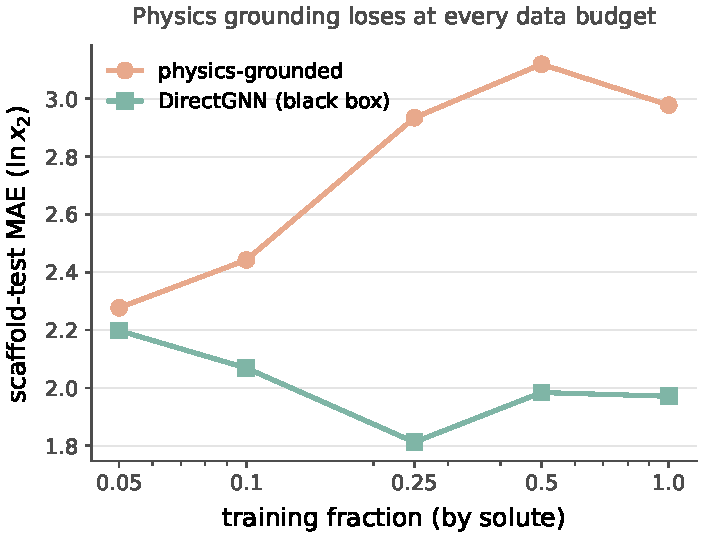
\includegraphics[width=\linewidth]{figs/fig_data_efficiency.pdf}
\caption[The data-efficiency curve]{Data-efficiency curve: scaffold-test MAE of the physics-grounded arm (salmon) and of
DirectGNN (teal) at five training-data fractions, one seed. The plotted values are the MAE columns
of Table~\ref{tab:data-eff}.}
\label{fig:data-eff}
\end{figure}


\section{A second chemical closure: pKa through a Hammett LFER}
\label{sec:pka}
% \S\ref{sec:pka-main} carries the statement of this result in the main text -- what was measured, on
% what, and the two signs. This appendix is the construction behind it and repeats those numbers on
% purpose; keep the two in step if either changes.
The measured result of this section is stated in \S\ref{sec:pka-main}; what follows is the
construction, the estimator and the sweep behind it.
The instrument is not specific to COSMO-SAC. In a second real domain---aqueous $\mathrm pK_a$ of
substituted aromatics---the fixed closure is a Hammett linear-free-energy relationship
$g(\zstar)=\mathrm pK_{a,0}-\rho\,\hammett^\star$ over $\zstar=(s,\hammett^\star)$: the reaction series $s$,
which fixes $(\mathrm pK_{a,0},\rho)$, together with the Hammett substituent constant \hammett,
written with its subscript throughout so that it cannot be confused with the $\sigma$-profile of
\S\ref{sec:framework}, with Hansch--Leo tabulated constants as the
external oracle. The two classic LFER failure modes fall cleanly onto the two channels of
Lemma~\ref{prop:decomp}: \emph{resonance saturation} (a curvature the linear closure cannot
represent) lands in $\Bclos$, while \emph{ortho/steric} effects, absent from the tabulated
constants, are information the intermediate lacks and land in $\Binsuf$. On the OPERA experimental
compilation \cite{mansouri2019opera}---the canonical full set under a uniform, closure-independent
quality filter that drops pre-ionized microstates (\S\ref{sec:si-pka})---this yields a
\emph{measured} fidelity sweep. The clean meta/para series ($n{=}158$) is well specified (RMSE $0.55$,
$\Bclos$ below the insufficiency floor). The degraded pole ($n{=}846$)---an ortho substituent, or one outside the tabulated
list, at some ring position (\S\ref{sec:pka-main})---degrades to
RMSE $2.26$, of which a within-series estimator conditioning on $(s,\hammett^\star)$ places at most $4.5$
of the $5.1$ total in input insufficiency and hence at least $0.6$ in the closure. That estimator is an out-of-fold residual, so
both figures are one-sided, and the a-priori
channel assignment---what the zeroed positions carry and the tabulated constant lacks---is consistent with the
measurement rather than established by it (\S\ref{sec:si-pka}); the sweep is the
near-exact-to-degraded transition. The decisive test is the
same oracle swap as on solubility---the learned $\hat\sigma_{\mathrm H}$ replaced by the tabulated $\sigma_{\mathrm H}^\star$
in the same closure, the sign of the change recorded per stratum---measured \emph{in-distribution} across
$K{=}20$ within-scaffold splits. It \emph{flips}. On the clean meta/para
pole feeding the reference constant \emph{helps} (learned MAE $0.48$ vs oracle $0.315$; oracle better
in $19/20$ splits and in three of the four reaction series): the ceiling there is the noisy learned estimate, not the
closure---a real-data pole on which grounding helps, and an internal positive control. On the degraded pole the
same swap \emph{hurts} (learned $0.83$ vs oracle $1.62$; oracle worse in $\mathbf{20/20}$ splits and in
all four series, gap $90\%$ CI $[{+}0.57,{+}0.95]$): the freely learned $\hat\sigma_{\mathrm H}$ absorbs what
the zeroed positions carry and the tabulated constant lacks. What reverses here is the sign of the grounding penalty; it
reverses through the insufficiency channel---consistent with the one-sided bound above, though not
isolated by it---rather than through the closure-error cancellation of \S\ref{sec:surrogate}: a second
instance of the sign rule, not of that mechanism.
The clustering unit is the Hammett reaction series, of which only $G{=}4$ exist,
so the accompanying bootstrap resolves nothing finer than series-level sign agreement---read as a
sign test on four units, $p{=}1/16$ on the degraded pole and $p{\approx}0.31$ on the clean one---and is
quoted as such (\S\ref{sec:si-pka}).

Both signs are one comparison: the sign of the grounding gap is by construction that of the learned
arm's error against the fidelity-set oracle error, and what a competence sweep adds is that the
oracle side of it does not move with the training budget while the learned side does
(\S\ref{sec:si-pka}). The well-specified pole's threshold (${\approx}0.315$) is never beaten by
the learned arm, so grounding helps at all four budgets swept. The degraded pole's threshold ($1.62$)
is high, so the learned arm beats it, and grounding hurts, across the whole interpolation range
(down to $12\%$ of the data), reverting to helps only under scaffold \emph{extrapolation}, where
$\hat\sigma_{\mathrm H}$ breaks ($2.6{\pm}2.0$) back above the threshold---in the mean over six
splits, three of which still have grounding hurting. The flip is thus a within-distribution, fidelity-driven crossover whose one
scope boundary is that same comparison read where the learned arm breaks. It is the sharp, two-sided form of the penalty sign rule
(Prop.~\ref{prop:tax}); its ``a fitted intermediate can beat the true one'' half is known---plug-in
efficiency under correct specification \cite{hirano2003}, pseudo-true fitting under misspecification
\cite{white1982}---sharpened here into a fidelity-set
threshold. The trained physics-vs-DirectGNN comparison is weaker and is not load-bearing
(\S\ref{sec:si-pka}). On an independent chemical closure the instrument separates a pole where
grounding helps from one where it hurts, each with a sign consistent across splits and series; the full construction,
the estimator validation and the measured sweep are in \S\ref{sec:si-pka} (Fig.~\ref{fig:pka}).

\section{The pKa closure: full construction, measured sweep, and trained comparison}
\label{sec:si-pka}
This section gives the full construction behind \S\ref{sec:pka}: a fixed
Hammett linear-free-energy relationship (LFER) $g(\hammett)=\mathrm pK_{a,0}-\rho\,\hammett$ over the
Hammett substituent constant $\hammett$ (with $\mathrm pK_{a,0},\rho$ the per-scaffold
Hansch--Leo--Taft reaction-series constants), for which Hansch--Leo tabulated constants provide an
external oracle $\zstar$. The analogy is close: as with the $\sigma$-profile through COSMO-SAC, a
learnable physical descriptor is pushed through a fixed, approximate, differentiable map. The two
classic LFER failure modes fall cleanly onto the two error channels of Lemma~\ref{prop:decomp}:
\emph{resonance saturation}---a curvature in $\hammett$ that the linear closure structurally cannot
represent---is a mis-map of a function of $\zstar$ and lands in $\Bclos$; \emph{ortho/steric} field
effects, absent from the tabulated constants, are information the intermediate lacks and land in
$\Binsuf$. The chemical scope is a fidelity sweep: meta/para monosubstituted benzoic acids, phenols,
and anilinium ions are the near-exact ($\Bclos\!\approx\!0$) regime, ortho
(insufficiency-dominated) and polyfunctional the low-fidelity one.

This decomposition is directly visible before any training. Pushed through the fixed Hammett
closure, $p$-nitrophenol reads $\mathrm pK_a\!\approx\!8.3$ against an experimental $\approx7.1$
(and $p$-nitroaniline overshoots similarly): the linear closure is off by $\sim1$ unit exactly
where through-conjugation ($\sigma_{\mathrm H}^-$) breaks it---$\Bclos$ observed in practice.

A controlled semi-synthetic construction on real tabulated $\hammett$ (known ground-truth
channels) validates the estimator and reproduces the paper's central distinction in this second
closure (Fig.~\ref{fig:pka}). Sweeping closure fidelity with a sufficient intermediate, the
grounding gap $\Ggap$ tracks $\Bclos$ (the plug-in estimate recovers the truth to within a few
percent, e.g.\ $0.20$ vs $0.21$, $0.81$ vs $0.81$), the case where Theorem~\ref{thm:gap}'s
proxy is valid. Sweeping the ortho/steric channel with a \emph{well-specified} closure gives
$\Bclos=0$ at every knob while $\Ggap$ rises with the insufficiency fraction, from $-0.035$ at zero
insufficiency through zero near a fraction of $0.25$ to $+0.34$ at $0.7$: at the three fractions
where it is positive it is positive with $\Bclos$ identically zero, which is the pKa realization of
the conflation that makes $\Ggap$ an indicator rather than a certificate. The two negative points
are the same statement in the other direction---a well-specified closure with a nearly sufficient
intermediate leaves the oracle marginally ahead. The oracle-$\hammett$ pipeline
(scaffold-resolved substituent$\to\hammett$ assignment) and this validation extend directly to real
data. On the OPERA experimental $\mathrm pK_a$ compilation \cite{mansouri2019opera} ($7{,}904$
records under the same net-neutral filter), applying the same decomposition to the fixed Hammett
closure yields a \emph{measured} fidelity sweep. On the clean meta/para series ($n{=}158$) the closure
predicts experimental $\mathrm pK_a$ to RMSE $0.55$, with the closure at the input-insufficiency floor:
the leakage-immune lower bound $\mathrm{MSE}-\Binsuf^{\mathrm{up}}$ is $-0.2$ ($95\%$~CI $[-0.4,-0.0]$),
i.e.\ below zero, as a lower bound on the non-negative $\Bclos$ must sit when the LFER predicts as well
as a flexible within-scaffold regressor. There $\Bclos$ is not separately resolvable and is consistent
with a well-specified closure (per-scaffold systematic offsets $\le0.18$). The ortho/heteroaromatic regime ($n{=}846$)
degrades to RMSE $2.26$, dominated by input insufficiency. Here the pKa latent is a \emph{scalar}
Hammett constant, so---unlike the solubility regime---$\Binsuf$ is estimated \emph{directly} rather
than through a coarsening of the closure's argument (\S\ref{sec:decomp}): a within-scaffold
out-of-fold regression estimator gives $\Binsuf=4.5$
($95\%$~CI $[4.0,5.1]$; $\approx89\%$ of the error---the tabulated $\hammett$ carries no ortho
information, exactly the a-priori channel assignment), leaving a closure misspecification
$\Bclos=0.6$ ($[0.3,0.8]$, a stratified within-scaffold molecule bootstrap). Directly estimated is
not point-identified: the estimator is an out-of-fold residual mean square, which is an upper
estimate of $\Ex[\Var(\mathrm{p}K_a\mid\hammett)]$, so $4.5$ is an upper figure and the $0.6$ it
leaves is a lower one---one-sided in the same direction as everywhere else in this paper, and
narrower only because the scalar latent needs no binning (\S\ref{sec:decomp},
\S\ref{sec:pka}). This is the
near-exact-to-degraded transition, measured rather than asserted. This places the pKa closure near the phase-diagram boundary
in its clean regime. \paragraph{Data quality control (uniform, closure-independent).} The trained runs use the canonical
full OPERA set ($7904$ records). A small number of entries are supplied as pre-ionized microstates---an
$[\mathrm{NH}^+]$-protonated aminopyridine at $\mathrm pK_a=-7.78$, a pyrylium $[\mathrm O^+]$, among
others---inconsistent with a neutral-scaffold Hammett assignment, and they degrade the clean pole
(pyridinium RMSE $0.63\!\to\!3.83$). We drop them with one rule, \emph{net formal charge} $\neq0$,
applied uniformly to both strata. It is closure-independent (it never references the oracle residual,
so it cannot be circular) and keeps net-neutral substituents such as nitro $[\mathrm N^+][\mathrm O^-]{=}\mathrm O$.
This removes $5$ of $163$ meta/para rows (restoring the clean pole to RMSE ${\approx}0.55$) and $352$
of $1198$ ortho rows (leaving $846$; the ortho RMSE is essentially unchanged, so the filter does not
manufacture the sign), for $1004$ Hammett-amenable rows.

\paragraph{Evidence for the flip.} We train the physics arm (encoder $\to\hat\sigma_{\mathrm H}\to$ fixed LFER)
on $K{=}20$ stratified $80/20$-within-scaffold splits---a Bemis--Murcko split collapses the meta/para
pole to two ring systems and is unstable---and record the paired per-molecule error against the
deterministic oracle, per stratum. Meta/para: learned MAE $0.48\pm0.09$ vs oracle $0.315\pm0.07$, gap
$-0.165$, oracle better in $19/20$ splits, $90\%$ CI $[-0.28,-0.04]$. Ortho: learned $0.83\pm0.07$ vs
oracle $1.62\pm0.08$, gap $+0.79$, oracle worse in $20/20$ splits, $90\%$ CI $[+0.57,+0.95]$ (both
intervals from the scaffold-cluster bootstrap).

\paragraph{What the two bootstraps do and do not resolve.} We report the sign statements above rather
than the bootstrap $P$ values, because neither bootstrap here carries the resolution a two-decimal $P$
implies. The cluster unit is the Hammett reaction series, and only $G{=}4$ exist (benzoic acid,
phenol, anilinium, pyridinium): the resampling law then has $\binom{7}{4}{=}35$ distinct outcomes and
a finest atom $(1/4)^4{\approx}0.004$, so the cluster-bootstrap $P(\text{oracle worse}){=}1.00$ on
ortho is exactly the statement that all four series means favour the learned arm, and $P{=}0.004$ on
meta/para that exactly one of them does, the other three favouring the oracle. Read as a sign test on
four units those are $p{=}1/16$ and $p{\approx}0.31$; the interval endpoints quoted above are
percentiles of the same $35$-outcome law and are no finer. This is the same small-$G$ caution applied
on the solubility side (\S\ref{sec:si-tables}), where the $P$ values are likewise read as a coarse
band rather than as two-decimal quantities. The split bootstrap adds nothing independent: the $20$
splits resample train/test assignments over the same molecules (each molecule lands in ${\approx}4$
test sets), so it prices split-to-split noise rather than molecule sampling, and with all $20$ ortho
gaps positive it returns $1.000$ by construction---a restatement of the $20/20$, not a second
confirmation. What the flip rests on is therefore the sign consistency across splits and series and
the size of the ortho gap ($+0.79$ against an oracle MAE of $1.62$, ${\approx}49\%$), not on a $P$
value. A leave-one-series-out refit, the estimate that would settle the series-level question at
$G{=}4$, was not run.

\paragraph{The crossover law and its scope boundary.} A competence sweep (train fraction
$\in\{1.0,0.5,0.25,0.12\}$ and, as the low-competence extreme, scaffold extrapolation; six seeds each)
confirms the sign is set by the crossover of the learned error against the fidelity-fixed oracle
threshold. On meta/para the learned arm rises from $0.46$ to $0.98$ as data shrinks but never reaches
the $0.31$ oracle threshold, so grounding helps throughout. On ortho the learned arm stays below the
$1.62$ threshold across the whole interpolation range ($0.85$ at full data, $1.31$ at $12\%$), so
grounding hurts throughout; only scaffold extrapolation, where $\hat\sigma_{\mathrm H}$ breaks to $2.6\pm2.0$,
pushes it back above the threshold and reverts the sign. The flip is therefore a within-distribution,
fidelity-driven crossover, and the extrapolation reversion is predicted by the same law. A trained
physics-vs-DirectGNN comparison agrees in direction overall but has weak absolute errors and an
untuned control; the load-bearing second-domain results are the decomposition above and the
sign-consistent flip.

\begin{figure*}[t]
\centering
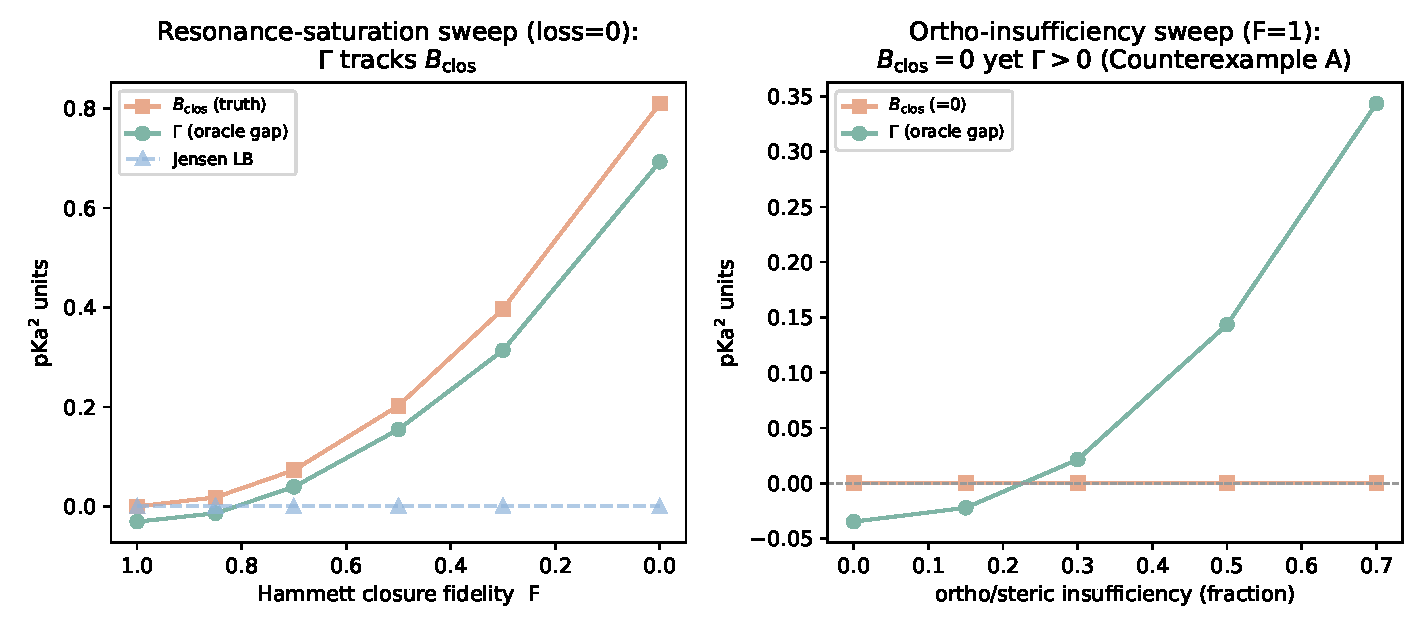
\includegraphics[width=\linewidth]{figs/fig_pka_hammett.pdf}
\caption{pKa through a Hammett LFER on a construction with known ground-truth
channels. \emph{Left:} closure fidelity varied with a sufficient intermediate; grounding gap
$\Ggap$, closure bias $\Bclos$, and the assumption-light Jensen bound. \emph{Right:} an
ortho/steric insufficiency channel varied with a \emph{well-specified} closure; $\Bclos=0$ at each
knob while $\Ggap$ rises with the insufficiency fraction, crossing zero near $0.25$.
Scope: \S\ref{sec:si-pka}.}
\label{fig:pka}
\end{figure*}


\subsection{Diagnostics that do not work, and why}
\label{sec:si-failed-diagnostics}

\begin{figure}[t]
\centering
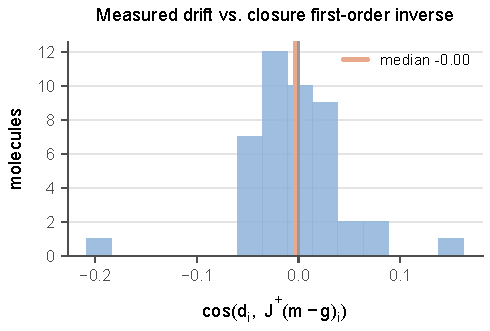
\includegraphics[width=0.82\linewidth]{figs/fig_picard_test.pdf}
\caption{Per-molecule cosine between the measured drift $\hat\sigma-\sigma$ and the first-order closure compensation
$J^{+}(m-g)$; the distribution is centred on zero (median $-0.00$).}
\label{fig:picard}
\end{figure}

\paragraph{The drift is not the closure's signed first-order inverse---but the test is under-resolved.}
A candidate account of the compensating drift is the closure's linear-response inverse,
$\hat\sigma-\sigma\approx J^{+}(m-g(\sigma))$ (with $J=\partial g/\partial\sigma$), predictable a priori
from $J$ before any solubility training. On the matched set the per-molecule drift shows no signed
alignment with $J^{+}(m-g)$ (median cosine $-0.00$; Fig.~\ref{fig:picard}).\footnote{The residual
COSMO-SAC closure runs a segment-activity fixed point, so its autograd Jacobian is numerically unstable
($\lVert\partial g/\partial\sigma_{\text{solvent}}\rVert\!\sim\!10^{15}$ at infinite dilution); $J$ is
computed by finite differences on the converged closure.} We read this as a signed negative only, and do
not build on it, for two reasons intrinsic to the test. First, the matched set is sparse (median one
pair per molecule), so each per-molecule Jacobian subspace is one-dimensional and the dimension-matched
row-space controls are uninformative---a resolved direction common across molecules makes a molecule's
``own'' and ``other'' subspaces coincide. Second, and more fundamentally, the single-pair $J^{+}(m-g)$
is a poor \emph{estimator} of the first-order compensation: the activity Fisher is near rank-one
($\mathrm{PR}\approx1.4$ of $51$, \S\ref{sec:surrogate}), so the closure's first-order inverse is
ill-posed along all but one direction. A null here is therefore uninformative about whether the drift is
first-order, not evidence that it is not. The load-bearing claim is the under-determination of $\sigma$
by activity (\S\ref{sec:surrogate}), not the geometry of the drift.

The instrument behind \S\ref{sec:surrogate}---the rank of the activity Fisher $J^{\top}J$
($J=\partial\lngi/\partial\sigma$), read as a participation ratio
$\mathrm{PR}=(\sum_i\lambda_i)^2/\sum_i\lambda_i^2$---is computationally inexpensive and oracle-free, which
is its appeal for probing any physics-grounded latent. It is also easy to misread in three ways that inflate a null or a rank
in the flattering direction, silently; we record them because the corrections are not obvious.

\paragraph{(i)~Finite differences inflate the participation ratio.} $\mathrm{PR}$ is a \emph{tail} statistic,
governed by the small eigenvalues. A closure evaluated by an unrolled fixed point carries a small,
step-\emph{independent} gradient noise (from the convergence tolerance, not truncation), so central finite
differences lift the exactly- and near-zero eigenvalues onto a floor and $\mathrm{PR}$ rises. On the
differentiable COSMO-SAC-2002 layer, autograd and finite differences on \emph{identical} profiles give
$\mathrm{PR}=1.00$ and $1.25$---a $25\%$ inflation from noise alone, though the per-gradient cosine is $0.995$
(the direction is right, the tail is not). It is worse on a typed ($3\times51$) profile basis: a closure that
ignores the typing (2002) has $102$ exactly-redundant coordinates that finite differences decorrelate into a
spurious floor, inflating its $\mathrm{PR}$ from $1.0$ toward $2.0$, while a closure that uses the typing
(2010) has no such redundancy---so the same step inflates the two \emph{asymmetrically} and can manufacture a
rank ordering with no physical content. \emph{Autograd is the appropriate instrument where the closure is
differentiable; with only finite differences, $\mathrm{PR}$ is interpretable against a known-rank or
permuted control, never absolutely.}

\paragraph{(ii)~``Own vs.\ other'' controls are powerless when the resolved direction is common.} A
dimension- and smoothness-matched control aligns a molecule's drift against its own predicted compensation and
against other molecules'. It has power only if the predictions differ. But when the aggregate Fisher is
rank-one (\S\ref{sec:surrogate}) the resolved direction is \emph{common}, so ``own'' and ``other'' point
almost the same way and the diagonal must sit inside the null---$p\approx0.5$ regardless of the truth. On the
matched set sparsity compounds this: a median of one pair per molecule makes each per-molecule Jacobian
subspace one-dimensional, so ``own'' and ``other'' subspaces coincide exactly. \emph{A control's null is
interpretable only once its power is established: if the compared predictions have median cosine near one,
the test cannot reject.}

\paragraph{(iii)~Energy-in-subspace baselines need the effective rank and a cluster null.} A random zero-mean
vector in $D$ dimensions places $k_{\mathrm{eff}}/(D{-}1)$ of its energy in a subspace of \emph{effective}
rank $k_{\mathrm{eff}}$ (the participation ratio of its singular values), which for near-collinear Jacobian
rows is far below the nominal row count. On the matched set the per-molecule subspace is effectively
one-dimensional, so the baseline is ${\approx}2\%$ and the observed $5.5\%$ is a two-to-threefold
\emph{enrichment}, not the ``no concentration'' a raw own-versus-other equality suggests: own equals other
because both one-dimensional subspaces are the same common direction, not because the drift avoids the
resolved one. And with that direction common, $N$ enriched molecules are not $N$ independent draws---the
enrichment needs a cluster null (\S\ref{sec:measure}), without which its significance is over-stated by
$\sqrt{N/N_{\mathrm{eff}}}$. We therefore report the $5.5\%$ as evidence in neither direction. \emph{The
baseline must be set by effective rank, and the null clustered by the shared direction.}

Each failure turns a soft spectral quantity into a hard structural claim---the mode the surviving
statements of \S\ref{sec:surrogate} avoid by carrying their null model and a power check inline.

\section{Data provenance and reproducibility}
\label{sec:si-repro}
\paragraph{Sources.} Solubility: BigSolDB~2.0 \cite{krasnov2025bigsoldb}. Crystal
$\Tm/\dHfus$: an open melting-point pool plus a group-contribution prior. True
$\sigma$-profiles: the VT-2005 database (ingested to
\texttt{sigma\_profiles.csv}, $1432$ compounds, with the COSMO cavity volume
$V_{\mathrm{cosmo}}$ for the combinatorial term). These are quantum-chemically computed for a
single reference conformer and protonation state; mismatch to the experimental measurement
conditions is noise in $\zstar$ that inflates $\Binsuf$, but under a Berkson-type displacement it
also loads onto $\Bclos$ through the curvature of $g$, so we treat it as an unsigned limitation and
\emph{not} as conservative for the closure-dominance verdict (\S\ref{sec:measure}). Infinite-dilution
activity coefficients: ThermoML. Enlarging the reference $\sigma$-profile set would not materially
grow the matched activity corner: of the $298$\,K ThermoML IDAC pairs, only two solutes lack a VT-2005
profile while their solvent has one---the binding constraint is joint IDAC$\times$profile coverage, not
profile availability. What does enlarge the corner is a broader extraction on the IDAC side: the
expanded ThermoML pull released with the code matches $115$ pairs at $298$\,K, which we do not adopt
because its verdict is quality-cut sensitive (\S\ref{sec:discussion}).
The corner is matched to VT-2005 by RDKit canonical SMILES on solute and
solvent, the rule the deployed $\sigma$-oracle itself uses; matching by InChIKey instead admits $85$
pairs over $46$ solutes and $19$ solvents at $298$\,K in place of $60/41/17$ (both counts are recorded
in \texttt{decomposition.json}). We keep the stricter rule so that the $\zstar$ charged against each
label is the profile the deployed pipeline would supply, rather than one imported across a tautomer or
protonation variant---the same mismatch that makes the reference imperfect above. The decomposition
was not re-estimated on the InChIKey-matched set; whether the verdict moves on those $25$ extra pairs
is untested. Second-domain pKa: the OPERA experimental compilation
\cite{mansouri2019opera} (\texttt{pKa\_QR.sdf}, $7904$ QSAR-ready records, public-domain US EPA;
cited, not redistributed); the uniform net-formal-charge filter reduces this to the $1004$
Hammett-amenable rows ($158$ meta/para, $846$ ortho/heteroaromatic) analysed in \S\ref{sec:si-pka}. The Bemis--Murcko scaffold split follows the main text; because the seeded
split is not stable across pipeline versions (\S\ref{sec:framework}), every number in this paper is
computed on a \emph{single} committed split, whose molecule-level hash is recorded with the released
artifacts.\footnote{The three-seed surrogate isolation (\S\ref{sec:surrogate}) was produced on a
separate run whose per-run split provenance was not logged; its matched set is the same $n{=}44$
molecules, derivable from the committed split independently of the model, so it is consistent with the
reported split. We record the split hash in the runner so future runs are auditable directly.}
Melting-point tables are auto-detected as $^\circ$C or K to avoid a $+273$\,K double-conversion.
% Artifact: notebooks/data/processed_sigma_aux_stream/summary.json (exclude_scaffolds_from points at
% a debug split; n_excluded_scaffolds 48 vs 2702 in the crystal stream's summary.json); guard in
% scripts/data/build_sigma_profile_aux_stream.py.
\paragraph{Grounding-stream provenance, and one build that violates the guard.} The
$\sigma$-stream builder drops any pool molecule whose Bemis--Murcko scaffold appears in the
validation or test split and aborts rather than proceed when a split file is missing; a correct
build retains $1319$ of the $1427$ VT-2005 molecules that parse into the pool. The stream file was
subsequently rebuilt with the exclusion pointed at the splits of a small debug dataset: it carries
$1425$ rows, of which $106$ ($99$ train, $7$ validation) have a scaffold in the real
test$\,\cup\,$validation union of $2702$ scaffolds. The overlap is not confined to scaffold
relatives: $91$ of those $106$ rows are themselves held-out solutes by canonical SMILES --- $65$
test solutes and $26$ validation solutes --- and the correctly guarded build leaves none of them.
The crystal stream's build on disk
records the correct $2702$-scaffold exclusion, so among the streams feeding the runs reported here
the defect is confined to the $\sigma$ one. Per-run stream provenance was not logged, so the
artifacts cannot certify which build fed which arm. The rebuilt file postdates every prediction file
behind Fig.~\ref{fig:paradox} and Table~\ref{tab:si-arms} and predates the two single-seed
oracle-application controls (\S\ref{sec:si-tables}) and the output-residual arms
(\S\ref{sec:gateb}); that ordering is consistent with the headline arms having used the guarded
build and the later controls the leaking one, but these are timestamps on local copies of
cloud-run outputs and settle nothing on their own. Three facts bound what the leak can do. It is
common-mode across the paradox contrast, the learned-$\sigma$ and $\sigma$-oracle rows being one
checkpoint evaluated two ways, so it cannot generate the gap between them; DirectGNN uses no
grounding stream, so a leak can only flatter the physics arm that loses to it; and on the $n{=}44$
matched set of \S\ref{sec:surrogate} a correct guard would have removed one molecule (piperidine).
What it does compromise is auditability, and with it the reach of the split guarantee: an arm
trained on that build would have had reference $\sigma$-profiles --- though no solubility labels ---
for $65$ test solutes, and the guarantee stated in \S\ref{sec:methods} is therefore a property of the
released builder rather than of every stream file we trained on. Closing this requires hashing each
stream build beside the split hash, which was not done for these runs.
\paragraph{Compute ledger.} The headline $\sigma$-grounding comparison
(Fig.~\ref{fig:paradox}, Table~\ref{tab:si-arms}) is a full-corpus GPU run (three seeds);
the closure/insufficiency decomposition (\S\ref{sec:measure}), the
Fisher audit (\S\ref{sec:ident}), the noise floor, the encoder probe, and the
temperature and mechanism diagnostics of \S\ref{sec:si-mech} are CPU-reproducible from
committed artifacts. Each figure and table names the script that regenerates it from
\texttt{results/}; large prediction CSVs and model checkpoints are deposited separately
(\pending[Zenodo DOI]) rather than in the repository.
\paragraph{Seeds and determinism.} Controlled comparisons use seeds $\{42,43,44\}$ and
are reported on a cross-arm intersection lock (rows supervised and finite in every arm); the
surrogate isolation (\S\ref{sec:surrogate}) uses seeds $\{0,1,2\}$; the training-time and
channel-swap oracle controls and the output-residual arms (\S\ref{sec:gateb}) are seed $42$ only.
The decomposition is seed-independent
(its closure has no learnable parameters). One artifact caveat: a save-time bug truncated the released
per-row prediction file for the seed-$44$ oracle solubility arm to $295$ rows, a small fraction of the
test set. The three-seed headline summaries (Fig.~\ref{fig:paradox}, Table~\ref{tab:si-arms}) were
aggregated at run time, before that file was written, so they are unaffected; only the one on-disk
artifact is partial, and any per-row re-analysis of the solubility arms therefore uses the two complete
seeds ($42,43$). The learned-$\sigma$ and DirectGNN solubility files and the activity-level
($n{=}60$, $n{=}44$) artifacts are complete for every seed.

\section{Black-box probe programme: full tables}
\label{sec:si-blackbox}
% Artifacts: results/blackbox/*.md and *.json; scripts/experiments/blackbox_study{1a,2,4}.py.
All three studies use the same current-split DirectGNN checkpoints (seeds $42/43/44$, test MAE
$1.749/1.674/1.684$) whose manifests pin the train/val/test SHA-256 to the split on disk. Every
figure is CPU-computed; no number here required a GPU.

\paragraph{Crystal-term decodability.} Probe fitted on $152$ solutes / $14{,}348$ rows,
scored on $13$ held-out solutes / $527$ rows, solute overlap zero. $\Phi^{*}$ is $92.2\%$
between-solute variance, so the effective $n$ is $13$ clusters.

\begin{table*}[t]
\centering\footnotesize
\begin{tabular}{lccccc}
\toprule
seed & $R^{2}$(model) & perm.\ $p$ & jackknife range & sign flips & top-3 leverage \\
\midrule
42 & $-0.506$ & $0.894$ & $[-1.151,\,-0.228]$ & $0/13$ & $56.2\%$ \\
43 & $+0.111$ & $0.055$ & $[-0.286,\,+0.333]$ & $3/13$ & $59.8\%$ \\
44 & $+0.027$ & $0.177$ & $[-0.253,\,+0.237]$ & $6/13$ & $57.2\%$ \\
\bottomrule
\end{tabular}
\caption{Crystal-term decodability per seed, with the permutation null, the drop-one-solute jackknife and the leverage carried by the worst solutes.}
\end{table*}

\noindent Controls: positive---model's own prediction $R^{2}=0.980$, temperature $R^{2}=0.9997$;
negative---random target $-0.0006$, molecule-blind constant profile $-0.015$, raw RDKit
descriptors $-0.514$ (set A) and $-0.928$ (set B). Null $p_{95}=+0.105/+0.117/+0.096$ and
$\max=+0.316/+0.380/+0.346$ over $1000$ draws.

Two features of this table bear on how such probes should be
read. First, the between-seed spread ($0.616$ range, sd $0.334$) exceeds every individual value:
a single-seed run would have been unreadable, and seed $43$ alone would have read as a
near-miss. Second, a decision rule of the common form
$R^{2}(\text{model})-R^{2}(\text{raw})\ge0.10$ would have declared success here on all three
seeds under descriptor set B---including seed $42$, whose probe is worse than a molecule-blind
constant---and on two of three under set A. The subtrahend is an unregistered analyst choice
worth more than the effect; we report $R^{2}(\text{raw})$ as a level beside $R^{2}$(model) and
never as a difference.

\paragraph{Temperature structure.} Slopes are fitted at fixed (solute, solvent); a slope
pooled across solvents would confound activity differences with temperature. Ceiling, measured on
the data before any model: $r=+0.239$ on train ($1353$ pairs / $151$ solutes) and $-0.125$ held
out ($66$ pairs / $13$ solutes, permutation $p=0.581$).

\begin{table*}[t]
\centering\footnotesize
\begin{tabular}{lccc}
\toprule
 & seed 42 & seed 43 & seed 44 \\
\midrule
corr(model, empirical slope) & $+0.294$ & $+0.406$ & $+0.195$ \\
corr(model, $-\Delta H/R$)   & $+0.066$ & $-0.283$ & $-0.028$ \\
median $|$model $-$ empirical$|$ slope & $1329$ & $1088$ & $1007$ \\
curvature in $1/T$ (data: $6.8\times10^{5}$) & $2.0\times10^{6}$ & $2.1\times10^{6}$ & $2.3\times10^{6}$ \\
\bottomrule
\end{tabular}
\caption{The model's temperature response against the empirical slope and against $-\Delta H_{\text{fus}}/R$, with the curvature of both in $1/T$.}
\end{table*}

\paragraph{Organisation of the representation.} Excess over a permutation null matched
to the factor's level, on the full test set.

\begin{table*}[t]
\centering\footnotesize
\begin{tabular}{lcccl}
\toprule
factor & seed 42 & seed 43 & seed 44 & null level \\
\midrule
solute identity (147 levels) & $+0.613$ & $+0.587$ & $+0.597$ & row \\
solute scaffold (124 levels) & $+0.614$ & $+0.586$ & $+0.595$ & row \\
scaffold beyond arbitrary solute grouping & $+0.082$ & $+0.082$ & $+0.082$ & solute \\
solvent identity (70 levels) & $+0.278$ & $+0.301$ & $+0.271$ & row \\
temperature & $+0.040$ & $+0.029$ & $+0.037$ & row \\
$\log P$ (solute) & $+0.089$ & $+0.048$ & $+0.028$ & solute \\
TPSA (solute) & $+0.060$ & $+0.061$ & $+0.042$ & solute \\
MolWt (solute) & $+0.032$ & $+0.013$ & $+0.018$ & solute \\
\bottomrule
\end{tabular}
\caption{Share of representation variance per organising factor, as an excess over a permutation null matched to the level at which that factor varies.}
\end{table*}

\noindent As a share of the solute-identity ceiling: scaffold $100.3/99.9/99.8\%$, $\log P$
$13.6/8.2/4.7\%$, TPSA $9.0/10.3/7.1\%$, MolWt $5.3/2.3/3.1\%$. The scaffold share is pinned near one
by the split rather than by the representation: only $34$ of the $147$ test solutes share a
Bemis--Murcko scaffold with another ($11$ multi-member scaffolds, $492$ of the $5608$ rows), so the two
partitions coincide on $91\%$ of the data. The raw variance shares in fact run the other way
(seed~$42$: scaffold $0.636$ against solute $0.639$), and the ratio reaches one only through the
differing size-matched permutation nulls ($0.022$ against $0.026$); no interval is attached to the
$0.2$--$0.9\%$ gap. The row therefore bounds what the representation adds beyond scaffold and does not
measure within-scaffold discriminability (\S\ref{sec:discussion}).

On the $331$ rows carrying a measured $\Phi^{*}$, $\Phi^{*}$ accounts for $18.3/42.5/18.0\%$ of
that subset's own solute-identity ceiling. This does not contradict the held-out null above.
$\Phi^{*}$ is a solute-level quantity and the representation is organised by solute identity, so
any solute-level variable shares variance with it in sample; the decodability probe above asks the different and
sharper question of whether the mapping transfers to solutes the probe never saw. In sample the
organisation is partly $\Phi^{*}$-aligned; out of sample that alignment does not carry.

\subsection{Closure fidelity sets the true-input penalty} \label{sec:dial}
% Artifact: results/synthetic_dial/summary.json via scripts/analysis/run_fidelity_dial.py (seed 0).
To isolate the mechanism behind the grounding paradox we built a controlled, reproducible
synthetic experiment in which the only quantity that varies is the fidelity of the closure,
with input quality, sample size, and estimator held fixed. A teacher draws a latent $\zstar$
and generates a target through a known map $T$; a fixed candidate closure $g_F$ reconstructs
the target from $\zstar$ under a tunable misspecification that deforms $T$ by a controlled
amount, summarized by a scalar fidelity $F$ ($F=1$ recovers $T$ exactly; $F$ decreases as the
closure is pushed further away). The measurement is the true-input penalty
$\Delta R^2 = R^2_{\text{oracle}}-R^2_{\text{head}}$, the change in fit from feeding the genuine
latent through $g_F$ rather than fitting a free head---$B_{\mathrm{closure}}$ made visible,
since the free head recovers $\Ex[m\mid\zstar]$ while $g_F$ is the misspecified map. As $F$
falls the penalty grows monotonically and without exception: averaged over six misspecification
functional forms (linear, quadratic, cubic, absolute-value, sinusoidal, cross-term), $F=1.00$
gives $\Delta R^2\approx0$; $F=0.76$ gives $\approx-0.04$; $F=0.38$ gives $\approx-0.33$; and an
over-rotation stress test ($F=-0.50$) gives $\approx-2.0$ (Fig~\ref{fig:dial}). The ordering is
identical across four unrelated teacher families---linear, monotone-nonlinear,
kinetics-exponential, and a PDE-field surrogate, agreeing to within a few hundredths at each
$F$---so the effect is a property of the fidelity magnitude, not of any one domain or
deformation form.

This construction separates the two error channels the physics path confounds. When the closure
is exact the true input is optimal and $\Delta R^2=0$; the penalty appears only as the closure
becomes misspecified, and its size is set by that misspecification alone. Placing the real system
on the same dial only illustratively---the mapping from a real closure to a scalar $F$ is a
synthetic construction, not an independently calibrated measurement---the COSMO-SAC closure over
predicted $\sigma$-profiles falls well inside the misspecified regime, where the dial's
solubility $\Delta R^2$ between the $\sigma$-oracle and learned-$\sigma$ arms ($\approx-0.36$)
lands at $F\lesssim0.4$ on the monotone curve. This locates the empirical grounding paradox on a
mechanistic axis: the loss from feeding true physical inputs is what one expects from a closure
of this fidelity, consistent with $\Bclos$ dominating $\Binsuf$.

The same engine also makes concrete why the grounding gap is a symptom rather than a certificate
(\S\ref{sec:gap}). With a knob on the sufficiency of $\zstar$, we can hold the closure
\emph{well specified} ($\Bclos=0$) and vary how much target-relevant information the intermediate
discards. When $\zstar$ is sufficient (A2 holds) the grounding gap $\Gamma$ tracks $\Bclos$ as
fidelity varies, the regime in which Theorem~\ref{thm:gap}'s proxy is exact; when $\zstar$ is
lossy but the closure is correct, $\Bclos=0$ throughout yet $\Gamma>0$ and grows with the
discarded variance (Fig~\ref{fig:conflation}). A positive grounding gap can therefore be pure
input insufficiency, not closure error---so the certificate of closure-dominance is the
convention-independent decomposition, and $\Gamma$ only corroborates it.

